\chapter{Nuclear Models}
\label{chapter-3}

In the following chapter, a discussion will be made about the nuclear models that are used in order to describe phenomena specific to rotating nuclei. Since the focus of this work emerges from a \emph{class} of properties that usually apply to the high-spin region, it makes sense to give an insight in the tools that cover all the underlying effects.

\section{Deformed Shell Model}

A formalism which describes the nuclear properties is the \emph{Shell Model}. It is based on an approximation of the independent motion for a nucleon within an average potential. The potential is generated by the interaction of that nucleon with all the remaining nucleons from the compounding nucleus. This formalism works really well for spherical nuclei and it is a successful tool in reproducing and predicting the properties of nuclear states. The theory also proves to be efficient for excited states having nucleonic configurations that are dominated by a single nucleon or a very small number of `extra' nucleons. However, this version of the Shell Model works well only for magic nuclei, nuclei that have both even number of protons and neutron, and nuclei whose shapes are not well deformed. In order to give a realistic description of a larger class of nuclei (e.g., deformed, odd $Z$, odd $N$, and so on), the \emph{Deformed Shell-Model} should be employed. This will be described in the following subsection, while a general overview of the concepts regarding the formerly mentioned model is made in Appendix \ref{appendix:shell-model}. Therein, the simple harmonic oscillator, and a modified version that is amended with additional terms are introduced. As it will be shown, these are used to obtain the Hamiltonian for the Deformed Shell Model.

% For nuclei that are even in both the proton number and the neutron number, the nuclear ground-state has a spin and parity that are properly reproduced by the \emph{spherical shell model}: $I^\pi=0^+$. In a nucleus with complete shells, the \emph{net spin} must be zero. On the other hand, a nucleus with one nucleon missing from a complete shell closure, the ground-state spin should be equal to the a.m. value of the orbital occupied by the hole. Moreover, the parity of the ground-state for a given nucleus is determined by the orbital a.m. value $l$:
% \begin{align}
%     \pi=(-)^l\to
%     \begin{cases}
%         +1 &\text{for even-}l\ \text{levels}\\
%         -1 &\text{for odd-}l\ \text{levels}\ .
%     \end{cases}
% \end{align}

% For odd-odd nuclei, one can find the ground-state (g.s.) spin and parity via the last two valence nucleons \cite{krane1991introductory,bertulani2007nuclear}. The coupling rules that are allowed in the odd-odd nuclei were determined more than 50 years ago by Gallagher et al. \cite{gallagher1958coupling}:
% \begin{align}
%     I&=j_p+j_n\ \text{if}\ j_p=l_p\pm\frac{1}{2}\ \text{and}\ j_n=l_n\pm\frac{1}{2}\ ,\\
%     I&=|j_p-j_n|\ \text{if}\ j_p=l_p\pm\frac{1}{2}\ \text{and}\ j_n=l_n\mp\frac{1}{2}\ .
% \end{align}

\subsection{Deformed Shell Model - Nilsson Model}
\label{nilsson-model-section}

The idea that some nuclei are deformed in their ground-state was enforced experimentally a long time ago when measuring quantities such as density distributions, nuclear quadrupole moments \cite{casten2000nuclear}. The non-spherical shapes are given by the existence of nucleonic configurations that lie away from the major shell closure. In Chapter \ref{chapter-2} the description of the nuclear shapes was treated, using the well-known formula for the parametrization of the nuclear radius in terms of the collective coordinates (see Eq. \ref{nuclear-shape}), resulting in the \emph{spherical}, \emph{axially-symmetric}, and \emph{axially-asymmetric} nuclear shapes.

Developed by Nilsson in 1955 \cite{nilsson1955binding} for treating the \emph{deformed nuclei}, it is a modified shell model with deformations taken into account by the use of the \emph{anisotropic harmonic oscillator} (AHO) (see Appendix \ref{appendix:shell-model} for the simple and modified ones). Similarly as for the basic shell model, the goal is to obtain an expression for the single-particle energies of a nucleon. The basic Hamiltonian corresponding to this kind of system is shown below \cite{bertulani2007nuclear}:
\begin{align}
    H=H_0+a_1\vec{l}\cdot\vec{s}+a_2l^2\ ,
    \label{nilsson-simple-hamiltonian}
\end{align}
where $H_0$ is the AHO term. The general expression for this kind of oscillator is:
\begin{align}
    H_\text{AHO}\equiv H_0=-\frac{\hbar^2}{2m}\nabla^2+\frac{1}{2}m(\omega_x^2x^2+\omega_y^2y^2+\omega_z^2z^2)\ .
\end{align}

In the expression of the single-particle Hamiltonian, the constants $a_1$ and $a_2$ are usually determined via adjustments to the experimental results. It can be seen that both the centrifugal-like term $l^2$, which simulates a flattening of the oscillator potential, and the $\vec{l}\cdot\vec{s}$ term are also present here, as it was the case for the spherical shell model. However, the explicit form of Eq. \ref{nilsson-simple-hamiltonian} is as follows:
\begin{align}
    H_\text{Nil}=-\frac{\hbar^2}{2m}\nabla^2+&\frac{1}{2}m(\omega_x^2x^2+\omega_y^2y^2+\omega_z^2z^2)-2\kappa\hbar\omega_0(\vec{l}\cdot\vec{s})\nonumber\\&-2\kappa\hbar\omega_0\mu\left(l^2-\langle l^2\rangle_N\right)\ .
    \label{eq-full-nilsson-ham}
\end{align}

The parameters $\kappa$ and $\mu$ act as strength parameters for the spin-orbit coupling term and the centrifugal term, respectively. The last term is a correction, which was introduced by Gustafson et al. \cite{gustafson1967nuclear}.
%The last term is a correction, which was originally considered as $\mu l^2$, but it was pointed by Gustafson et al. \cite{gustafson1967nuclear} that the shift in energy is way too large for big values of $N$ (principal quantum number). As a result, taking the current expression for the correction term helps to compensate.
The three \emph{oscillator frequencies} are chosen to be inversely proportional to the semi-axis lengths of the deformed ellipsoid (denoted by $a_x$, $a_y$, and $a_z$) such that:
\begin{align}
    \omega_r=\omega_0\frac{R_0}{a_r}\ ,\ r=x,y,z\ .
\end{align}

For the spherical case, the oscillator frequency $\hbar\omega_0$ is set to $41A^{-1/3}$ MeV (calculation for this value arise from the shell model with SHO \cite{bertulani2007nuclear}). For the axially-symmetric case, one can choose the $z$-axis as symmetry axis, implying that the oscillator frequencies along the $x$ and $y$ axes are equivalent (that is $\omega_x=\omega_y\equiv\omega_\perp$). Following the calculations done in \cite{bertulani2007nuclear}, one can express the two relevant oscillator frequencies in terms of a deformation parameter $\epsilon_2$ (whose dependence on the quadrupole deformation parameter $\beta_2$ has been shown in Eq. \ref{epsilon-beta-relation}) as such:
\begin{align}
    \omega_\perp^2=\omega_0^2\left(1+\frac{2}{3}\epsilon_2\right)\ ,\\
    \omega_z^2=\omega_0^2\left(1-\frac{4}{3}\epsilon_2\right)\ .
    \label{oscillator-frequencies-nilsson}
\end{align}

Moreover, a dependence on the deformation parameter itself is employed for the frequency $\omega_0$ that appears in the expressions for $\omega_\perp$ and $\omega_z$, respectively:
\begin{align}
    \omega_0=\left(1-\frac{4}{3}\epsilon_2^2-\frac{16}{27}\epsilon_2^3\right)^{-1/6}\ ,
    \label{omega-0-oscillator-frequency}
\end{align}
where $\bar{\omega}_0$ can be considered a constant written as $\bar{\omega}_0=(\omega_x\omega_y\omega_z)^{1/3}=\text{const}$. This is coming from the harmonic oscillator at zero deformation and by considering the conservation of the nuclear volume. The energy eigenvalue $\varepsilon_q$ for the nucleonic state $\psi_q$ belonging to a deformed nucleus can be determined by solving the Schrödinger equation associated to each nucleon in particular:
\begin{align}
    H_\text{Nil}\psi_q=\varepsilon_q\psi_q\ ,
    \label{nilsson-schrodiner-equation}
\end{align}
where the index $q$ denotes a set with all the relevant quantum numbers. This set is also called the \emph{asymptotic quantum numbers}, which are used to specify a \emph{Nilsson orbital}. The well-known notation is as follows (still considering the $z$-axis as the symmetry axis):
\begin{align}
    \Omega^\pi\left[Nn_z\Lambda\right]\ .
    \label{nilsson-notation}
\end{align}
\begin{itemize}
    \item $\Lambda$ is the projection of the particle's orbital a.m. along the symmetry axis (component of $l$ along $z$)
    \item $N$ the principal quantum number of the major shell. It also determines the parity as $\pi=(-1)^N$, making the notation from Eq. \ref{nilsson-notation} somewhat redundant
    \item $n_z$ is the number of oscillator quanta along the symmetry axis. More precisely, it gives the number of nodes for the wave-function along the direction of the $z$-axis
    \item $\Omega$ is the projection of the particle's total a.m. along the symmetry axis (i.e., $\mathbf{j}$). Moreover, the projection of the intrinsic spin of a nucleon onto the symmetry axis can have the values $\Sigma=\pm\frac{1}{2}$, so that $\Omega=\Lambda+\Sigma=\pm\frac{1}{2}$.
\end{itemize}

Fig. \ref{fig-nilsson-quantum-numbers} shows the geometrical meaning of the asymptotic quantum numbers for the Nilsson model. Indeed, for a single nucleon orbiting a deformed core, the vector $\mathbf{R}$ represents the angular momentum of a \emph{rotating nucleus}, the vector $\mathbf{I}$ represents the total a.m. of the entire nucleus, $\mathbf{j}$ is the total a.m. of the single-particle (that is $\mathbf{j}=\mathbf{l}+\mathbf{s}$). However, two more quantum numbers should be mentioned: the projection of the total a.m. $\mathbf{I}$ onto the symmetry axis, denoted by $K$, and the projection of the same vector onto the laboratory axis, referred to as $M$.
\begin{figure}
    \centering
    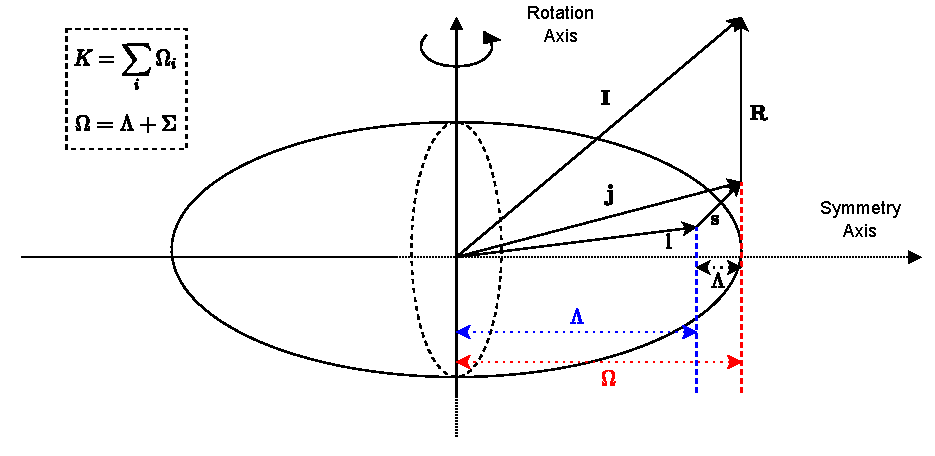
\includegraphics[width=0.99\textwidth]{Chapters/Figures/nilsson_quantum_numbers.pdf}
    \caption{A schematic showing a geometrical interpretation of the Nilsson's asymptotic quantum numbers. This figure is inspired from Ref. \cite{garnsworthy2007neutron}}
    \label{fig-nilsson-quantum-numbers}
\end{figure}

Regarding the quantum numbers sketched in Fig. \ref{fig-nilsson-quantum-numbers}, there is an important aspect which needs to be specified about the projections $K$ and $\Omega$, respectively. Indeed, it is clear that compared to the spherical case, where different orientations are irrelevant to the energy spectrum of nucleons, in the deformed case different directions in space lead to different energies. The orientation is in fact specified by the \emph{magnetic sub-state} of the nucleon, i.e., the projection of the total angular momentum on the symmetry axis. This projections is denoted by $\Omega$ for the single-particle, however, because the rotational angular momentum $\mathbf{R}$ in the axially deformed is perpendicular to the symmetry axis for low-lying states, then it will have no contribution to $K$, meaning that one can use $\Omega$ and $K$ interchangeably.

\subsection{Single-particle states in deformed nuclei}

It is instructive to go into detail about the quantum numbers defined in Eq. \ref{nilsson-notation}, since the orbits characterizing the nucleons point out the nature of deformations that take place. The quantum numbers $N$, $n_z$, and $\Lambda$ are good quantum numbers only when the nuclear deformation is large, meaning that $\epsilon$ (or equivalently $\beta$) tends to infinity. In fact, this is the main reason why they are called asymptotic quantum numbers. However, the numbers $\Omega$ and $\pi$ remain good quantum numbers even for low and moderate deformations for the nucleus. It should be noted that if $N$ is even, then $(\Lambda+n_z)$ is also even. Similarly, if $N$ is odd, then the sum of the other two quantum numbers must also be odd \cite{casten2000nuclear}.

Since the eigenvalues of the Hamiltonian $H_\text{Nil}$ ultimately depend on the deformation parameter $\epsilon$, each nucleon will have an orbit (energy) that is deformation dependent. At no deformation, all the energy levels for a single-particle state will have a $2j+1$ degeneracy. This translates to the fact that all $2j+1$ possible orientations of $\vec{j}$ are equivalent. On the other side, when the potential is deformed, this will no longer hold, i.e., the energy levels in the deformed potential will depend on the spatial orientation of the orbit itself.

As an example, a nucleon from the $f_{7/2}$ shell will be considered. This nucleon can have eight possible components in the range $\Omega=[-\frac{7}{2},\frac{7}{2}]$. Because of the reflection symmetry, the positive components of $\Omega$ will have the same energy as the negative ones, leading to a degeneracy of the levels. Additionally, the single-particle $f_{7/2}$ state will split up into four new states when deformation emerges: $\Omega=\frac{1}{2},\frac{3}{2},\frac{5}{2},\frac{7}{2}$ (all of negative parity). In Figs. \ref{nillson-orbits-prolate-projections} - \ref{nillson-orbits-oblate-projections} the different orbits of the odd particle are given for both prolate and oblate deformations.
\begin{figure}
    \centering
    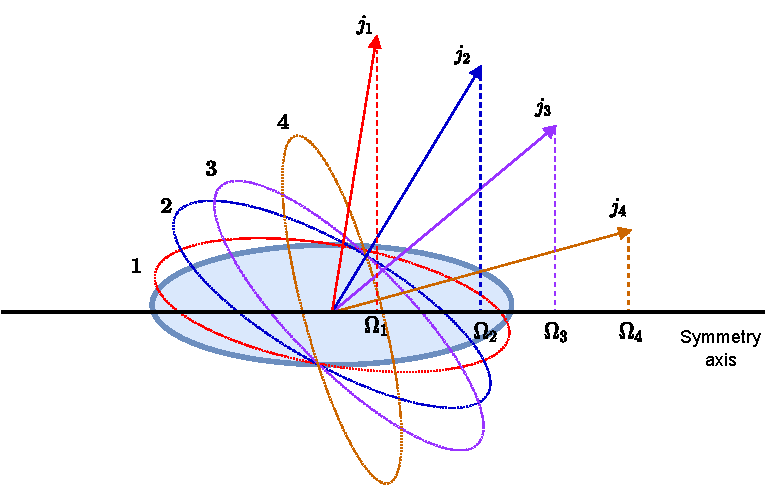
\includegraphics[scale=1]{Chapters/Figures/nillson_SP_orbits.pdf}
    \caption{A simple sketch showing the single-particle orbits for the $j=7/2$ nucleonic state, along the symmetry axis for a \emph{prolate} deformation. The actual projections are $\Omega_1=\frac{1}{2}$, $\Omega_2=\frac{3}{2}$, $\Omega_3=\frac{5}{2}$, and $\Omega_4=\frac{7}{2}$. The figure was inspired from Ref. \cite{krane1991introductory}.}
    \label{nillson-orbits-prolate-projections}
\end{figure}
\begin{figure}
    \centering
    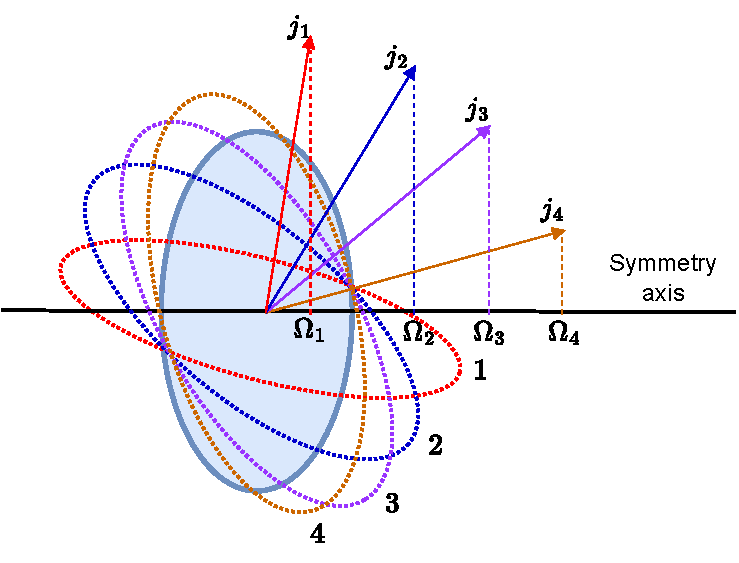
\includegraphics[scale=1]{Chapters/Figures/nillson_SP_orbits_2.pdf}
    \caption{A simple sketch showing the single-particle orbits for the $j=7/2$ nucleonic state, along the symmetry axis for an \emph{oblate} deformation. The actual projections are $\Omega_1=\frac{1}{2}$, $\Omega_2=\frac{3}{2}$, $\Omega_3=\frac{5}{2}$, and $\Omega_4=\frac{7}{2}$. The figure was inspired from Ref. \cite{krane1991introductory}.}
    \label{nillson-orbits-oblate-projections}
\end{figure}

From Figs. \ref{nillson-orbits-prolate-projections} - \ref{nillson-orbits-oblate-projections}, it can be seen that the first orbit (denoted by orbit $1$) lies closest to the core in the prolate case, while in the oblate case this is true for orbit $4$. This will influence the interaction strength, meaning that for the prolate case, the orbit $1$ will interact the strongest with the \emph{core}, while in the oblate case, it is the orbit $4$ having the strongest interaction with the bulk core. Moreover, the strength of interaction indicates the magnitude of the energies for each projection: the stronger the interaction between the orbit and the core, the more tightly bound and lower in energy these states are. For prolate deformations, the orbits with the smallest $\Omega$ `prefer' to lie lower in energy (interacting strongly with the core). For oblate deformations, the opposite is true: orbits with the maximal $\Omega$ interact the strongest with the core and, therefore, lie lowest in energy.

Another way of looking at the coupling of the single-particle with the bulk core can be given in terms of overlaps of their corresponding wave-functions (eigenstates). Indeed, a nucleon lying in the lowest $\Omega$ orbit will have a \emph{maximum} wave-function overlap with a prolate core. On the other hand, nucleons lying in the highest $\Omega$ orbits will have maximum overlap with the oblate core. The overlap gives the overall binding energy between the two systems (i.e., core and particle) as explained in the previous paragraph. Discussion about the wave-function overlap and the nuclear density distribution \cite{frauendorf2014transverse, das2018nuclear} will be made in the following chapters. The induced degeneracy due to deformation for a particle state $l_j$ is shown in Fig. \ref{nillson-orbits-splittings}, for $f_{7/2}$.
\begin{figure}
    \centering
    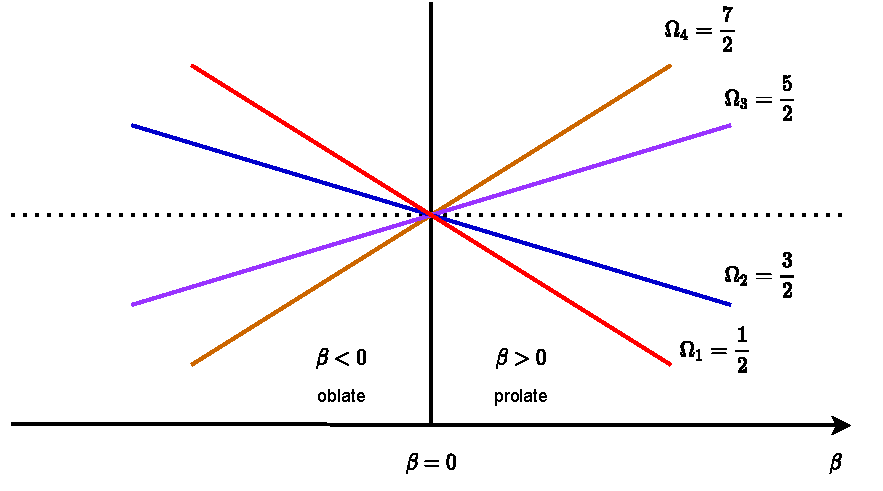
\includegraphics[width=0.99\textwidth]{Chapters/Figures/nillson_SP_splittings.pdf}
    \caption{The effect of deformation for the particle state $f_{7/2}$. It can be seen that indeed, as it was mentioned within the text, $\Omega_1$ component lies lowest in energy for the oblate deformation, and $\Omega_4$ component lies the lowest in energy for an oblate deformation.}
    \label{nillson-orbits-splittings}
\end{figure}

Obviously, the sketch shown in Fig. \ref{nillson-orbits-splittings} is just an instructive example, and it does not represent an accurate description of the single-particle energies for deformed nuclei. In fact, if the potential is deformed, the quantum numbers $l$ and $j$ are not valid anymore (a.m. is no longer a constant of motion for non-spherical potentials). A proper description of the single-particle orbits is represented by the so-called \emph{Nilsson diagrams}, where the energy for each state is represented as a function of the deformation parameter. Remember that the energies are in fact the eigenvalues of the Schrödinger equation associated with the initial Nilsson deformed Hamiltonian (see Eq. \ref{nilsson-schrodiner-equation}). Diagrams that show such spectra are represented in Figs. \ref{nillson-diagram} - \ref{nillson-diagram-2}. It can be seen that each state within a Nilsson diagram is represented as a solid line or a dashed line, depending on its parity (remember that the parity quantum number is given by $(-1)^N$ or, equivalently, by $(-1)^l$). The orbital labelling from the Figs. \ref{nillson-diagram} - \ref{nillson-diagram-2} is consistent with the one defined in the previous subsection. Another important aspect which can be seen in the Nilsson diagrams (for some orbits) is the `crossing' between states with different quantum numbers. More insight into the geometrical interpretation of the Nilsson orbitals is provided in Section \ref{appendix:extra-nilsson-orbitals} from Appendix \ref{appendix:shell-model}.

% The spectrum of one-particle orbits plays an invaluable role within the nuclear structure and the study of deformations: the picture of one-particle motion in deformed potentials works much better than the case of single-particle motion in spherical potentials for spherically shaped nuclei. Multiple quantitative analyses have been performed on experimental data of well-deformed (especially odd-$A$) nuclei, from light ($^{25}$Mg, $^{25}$Al) to heavy ($^{169}$Tm, $^{175}$Yb, $^{177}$Yb) \cite{hamamoto2016interplay}.
\begin{figure}
    \centering
    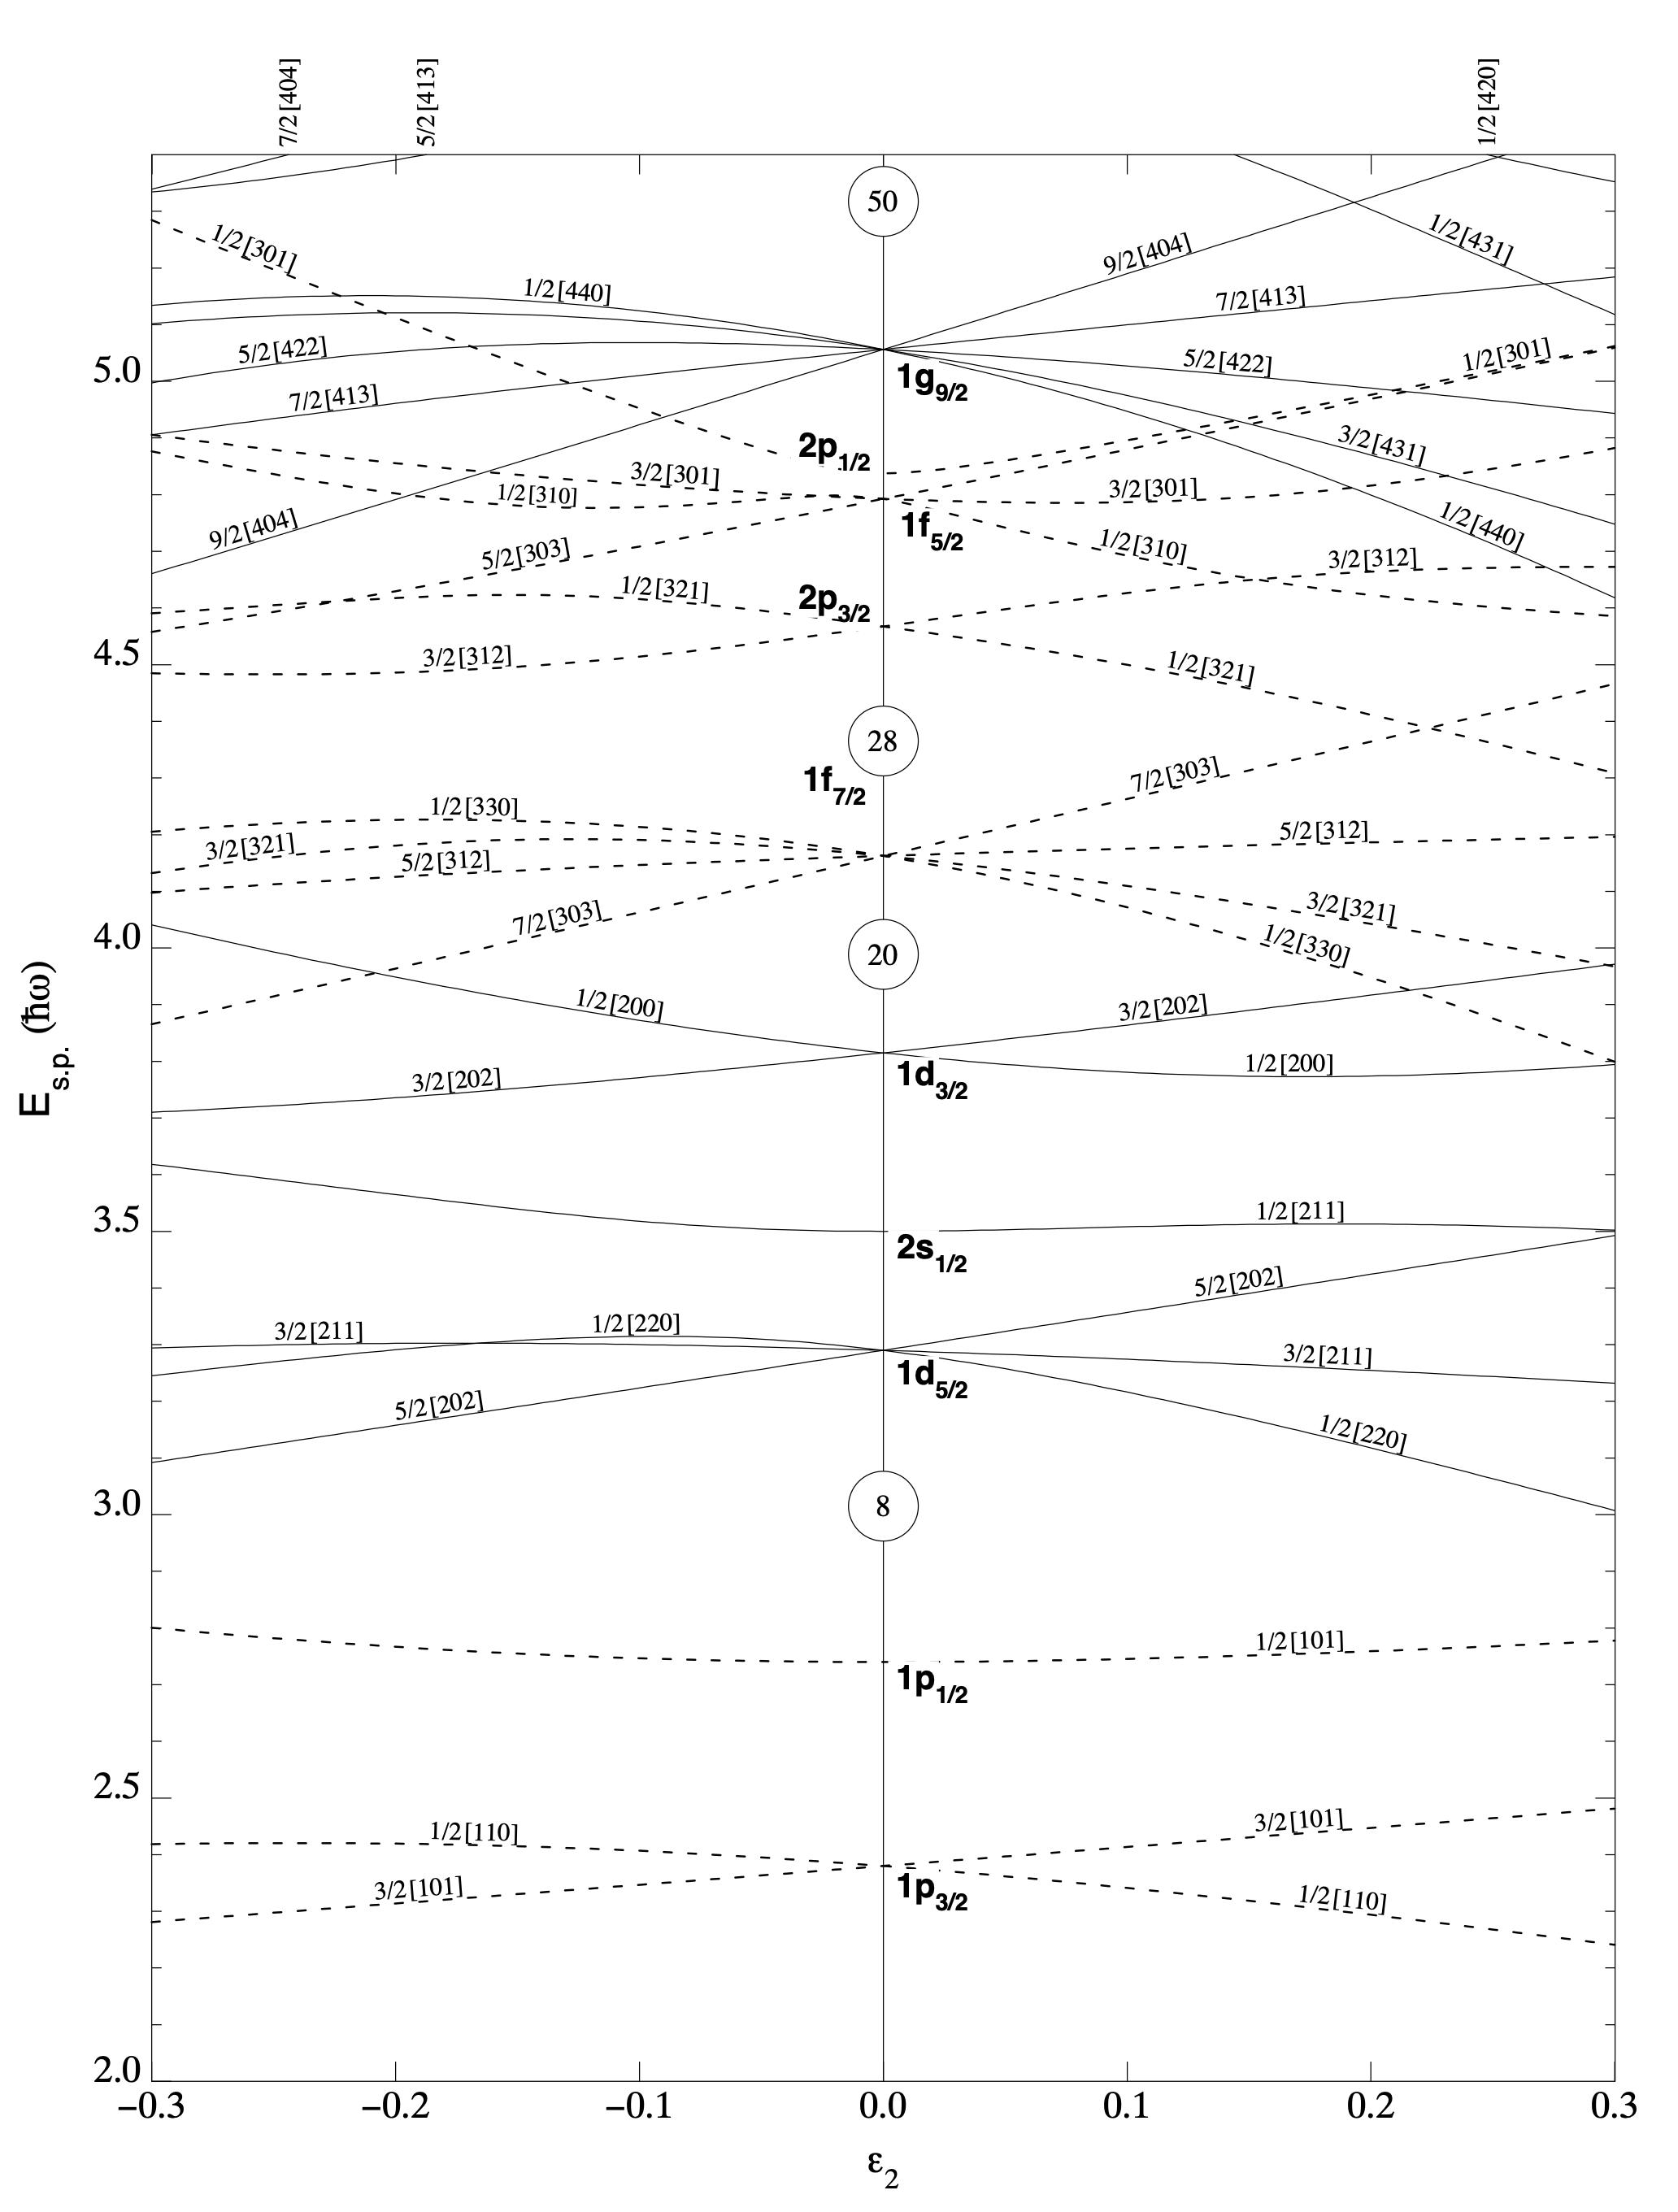
\includegraphics[width=0.99\textwidth]{Chapters/Figures/nillson_diagram.png}
    \caption{A Nilsson diagram for protons or neutrons, with $Z$ or $N\leq50$. Picture taken from Ref. \cite{ragnarsson2005shapes}.}
    \label{nillson-diagram}
\end{figure}
\begin{figure}
    \centering
    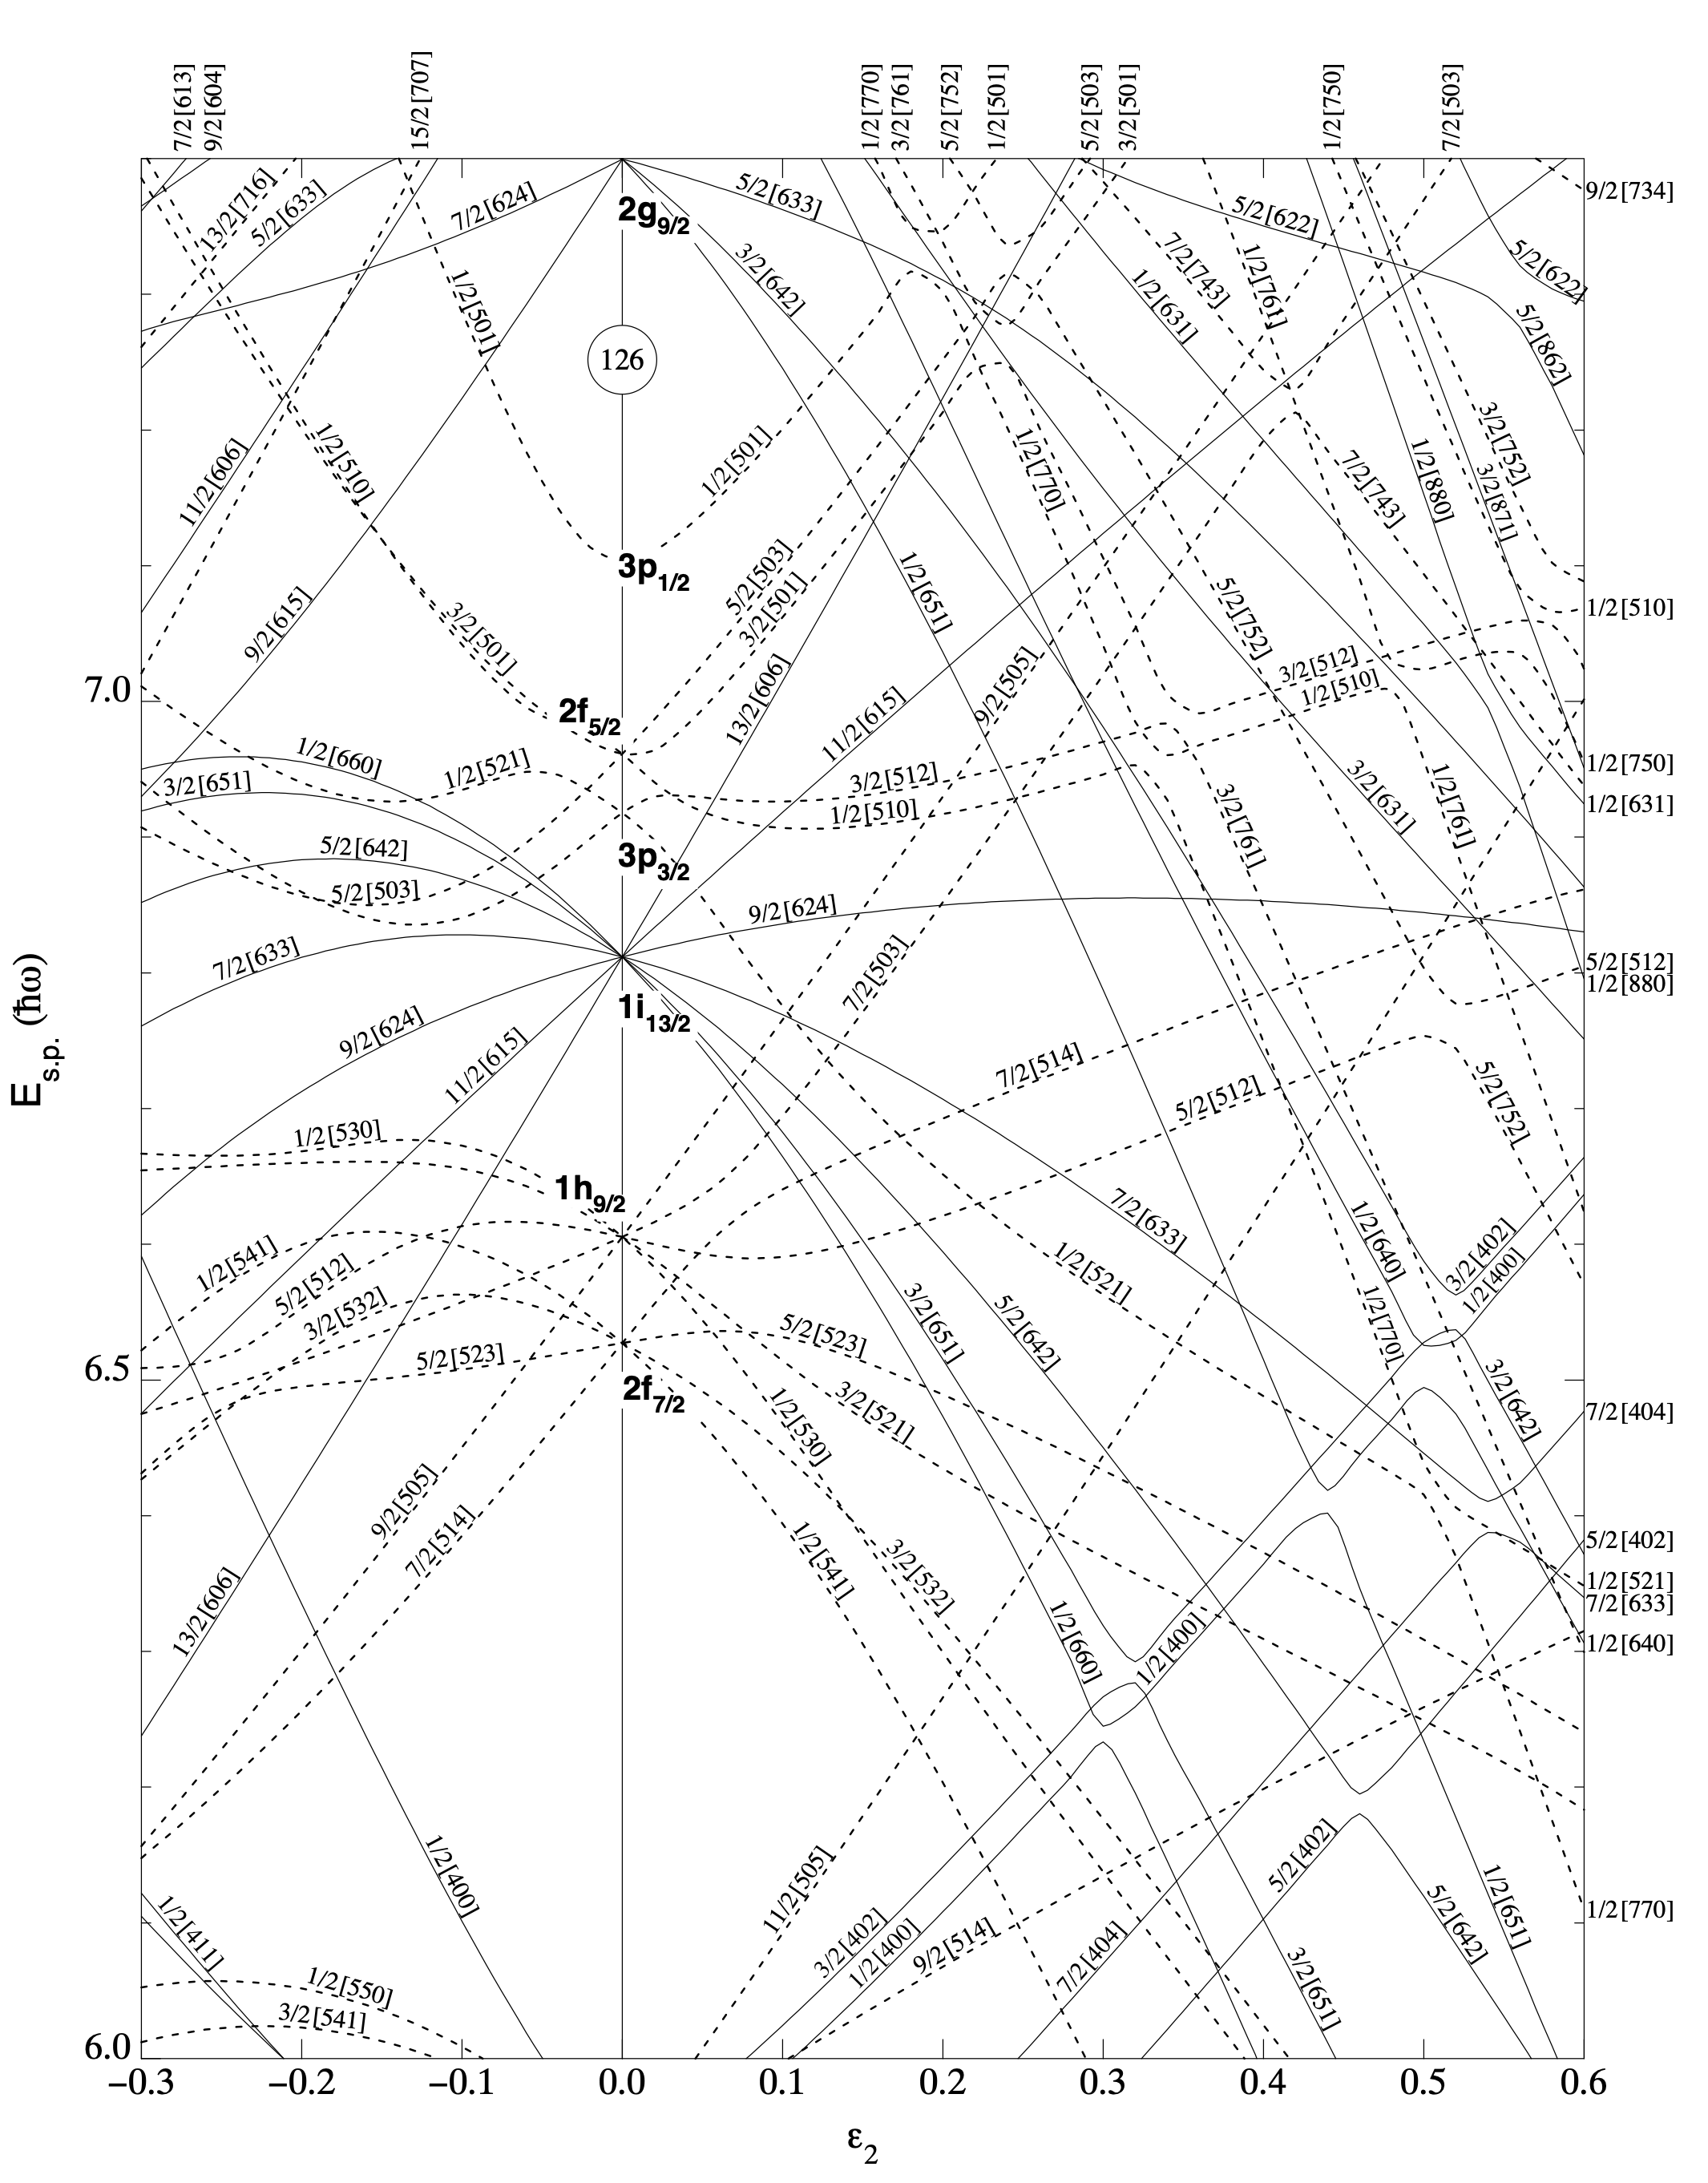
\includegraphics[width=0.99\textwidth]{Chapters/Figures/nillson_diagram_2.png}
    \caption{A Nilsson diagram for neutrons, with $82\leq N\leq126$. Picture taken from Ref. \cite{ragnarsson2005shapes}.}
    \label{nillson-diagram-2}
\end{figure}

\pagebreak

\section{Collective Model}

Although the previous single-particle model is able to successfully treat many nuclei, the single-nucleon motion in a deformed potential is not enough to describe phenomena such as nuclear fission or quantities like quadrupole moments of deformed nuclei \cite{townes1949nuclear}. Moreover, lifetime measurements through single-particle calculations fail to reproduce experimental data on some gamma-ray transitions of quadrupole nature \cite{goldhaber1951classification}.

The collective model is one of the most `complete' tools in describing the nuclear phenomena across the chart of nuclides. It brought tremendous progress within the nuclear community by validating and predicting the nuclear behavior at different spin ranges. A major feature of this model is the introduction of the so-called \emph{rotational bands}. Developed by Bohr and Mottelson \cite{bohr1953collective,bohr1998nuclear} more than 50 years ago, the Nuclear Collective Model is based on the Liquid-Drop-Model \cite{meitner1939disintegration,bohr1939mechanism,myers1974nuclear}. Moreover, the predictions for nuclear deformation made by Rainwater \cite{rainwater1950nuclear} played another fundamental role. The basic assumption is that the nuclear density distribution can be approximated as a droplet with shape-specific degrees of freedom. This droplet is also vibrating and rotating. According to the discussion from Chapter \ref{chapter-2}, the nuclear radius was described in terms of a set of \emph{collective coordinates}, which dictate the shape evolution with time.

\subsection{Bohr Hamiltonian}

As a first step, the concept of a nuclear liquid drop is used to construct the Hamiltonian. The droplet exhibits shape and surface oscillations, which have a dynamical character. These shape oscillations are illustrated in Fig. \ref{fig-nuclear-vibration}, where a vibrating nucleus is represented, having a spherical \emph{equilibrium} shape. Since the collective coordinates are time-dependent, at each moment in time, the nuclear radius $R$ will be defined in the direction given by the radial coordinates $\theta,\varphi$. By using Eq. \ref{nuclear-shape} that characterizes the \emph{vibrations} of a nuclear surface, one can give the Hamiltonian of \emph{collective} nature as \cite{ring2004nuclear,bertulani2007nuclear}:
\begin{align}
    H_\text{coll}\equiv T+V=\frac{1}{2}\sum_{\lambda\mu}\left[B_\lambda\left|\frac{\text{d}\alpha_{\lambda\mu}}{\text{d}t}\right|^2+C_\lambda|\alpha_{\lambda\mu}|^2\right]\ .
    \label{collective-hamiltonian-stiffness-inertia}
\end{align}
\begin{figure}
    \centering
    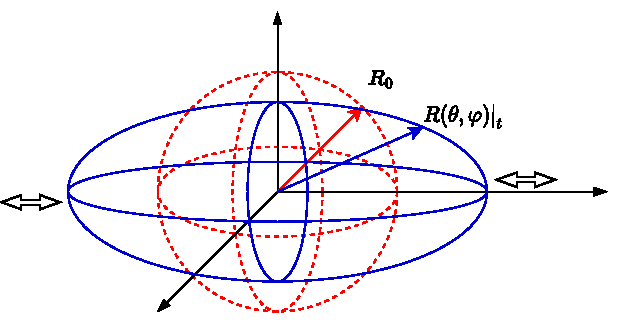
\includegraphics[width=0.99\textwidth]{Chapters/Figures/shape_oscillations.pdf}
    \caption{The vibration of a nucleus whose equilibrium shape is a spheroid, with nuclear radius $R_0$ (\emph{average nuclear radius}) and the nuclear radius $R$ at a different moment in time. The equilibrium shape is represented by the red color, while the surface vibration is represented by the blue color. The oscillations are depicted through the double arrows.}
    \label{fig-nuclear-vibration}
\end{figure}

The Hamiltonian is invariant under rotations and also invariant under time reversal \cite{messiah2014quantum}. The real numbers $B_\lambda$ and $C_\lambda$ represent the \emph{inertial} and \emph{stiffness} parameters. Choosing the body-fixed axis as a reference system will simplify the results, since the system's axes coincide with the principal axes of the ellipsoid itself. Assuming this coordinate system and an axial ellipsoid, the kinetic term from $H_\text{coll}$ can be decomposed into a \emph{rotational} and a \emph{vibrational} part, i.e., $T=T_\text{vib}+T_\text{rot}$. Their expressions are given in terms of the deformation parameters $(\beta,\gamma)$, the mass parameters $B_2$ (for the quadrupole deformations) and the stiffness parameters $C_2$. Thus, the vibrational term is \cite{li2022model}:
\begin{align}
    T_\text{vib}=\frac{1}{2}B_2\left(\dot{\beta}^2+\beta^2\dot{\gamma}^2\right)\ ,
    \label{kinetic-vibrational-energy-collective}
\end{align}
and the rotational term is \cite{li2022model}:
\begin{align}
    T_\text{rot}=\frac{1}{2}\sum_i^3\mathcal{I}_i\omega_i^2\ ,
    \label{kinetic-rotational-energy-collective}
\end{align}
where the three principal axes of the ellipsoid are indexed by $i=1,2,3$. In the expression of $T_\text{rot}$, two crucial physical quantities arise, namely the angular velocities around each body-fixed axis and the functions $\mathcal{I}_k$ that will eventually play the role of \emph{moments of inertia}. 

There are two types of moments of inertia that describe the nuclear rotation: the rigid-like MOI and the irrotational (hydrodynamical) MOI, having the following expressions \cite{bohr1954rotational,ring2004nuclear}:
\begin{align}
    \mathcal{I}_k^\text{rig}&=\frac{2}{5}mAR_0^2\left(1-\sqrt{\frac{5}{4\pi}\beta\cos\left(\gamma-\frac{2\pi}{3}k\right)}\right)\ ,\\
    \mathcal{I}_k^\text{irr}&=\frac{3}{2\pi}mAR_0^2\beta^2\sin^2\left(\gamma-\frac{2\pi}{3}k\right)\ .
    \label{eq-irrotational-rigid-mois}
\end{align}

The dependence of the two types of MOI on the triaxiality parameter $\gamma$ (and fixed $\beta$) can be seen in Fig. \ref{fig-irrotational-rigid-mois}. The differences between the rigid and irrotational MOI are as follow:
\begin{itemize}
    \item The irrotational MOI vanish when the ellipsoid has axial symmetry
    \item $\mathcal{I}^\text{irr}$ is much more sensitive to the deformation $\beta$, while the rigid MOI have most of the contribution coming from a typical rigid sphere
    \item The \emph{experimental} MOI of well-deformed nuclei show that the \emph{real} MOI within a nucleus are neither irrotational, nor rigid-like, but in fact they follow:
    \begin{align}
        \mathcal{I}^\text{irr}<\mathcal{I}^\text{exp}<\mathcal{I}^\text{rig}\ ,
        \label{experimental-MOI-vs-rig-irr}
    \end{align}
\end{itemize}
\begin{figure}
    \centering
    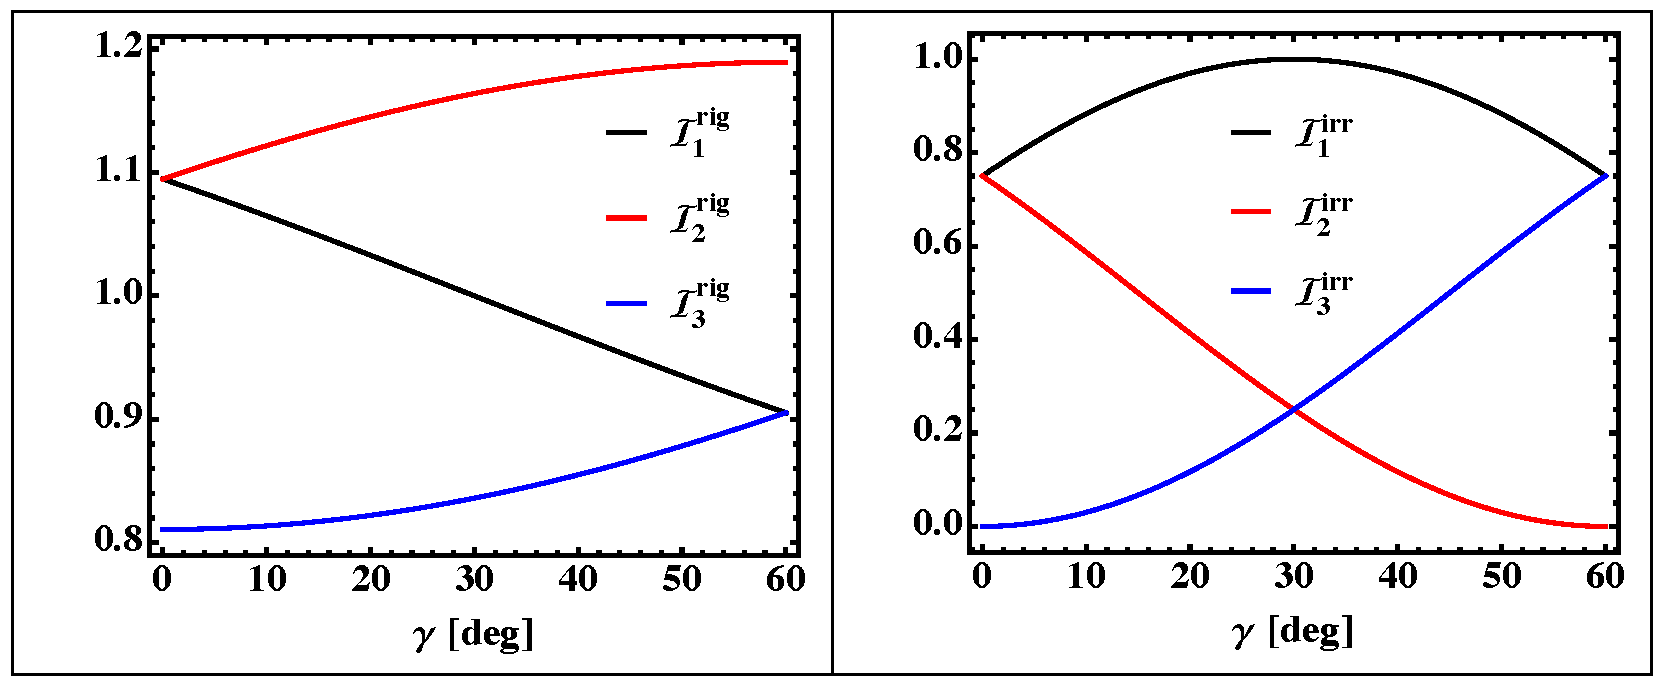
\includegraphics[width=0.99\textwidth]{Chapters/Figures/mois_rig_irr.pdf}
    \caption{Comparison between the rigid-like and irrotational-like MOI defined in Eq. \ref{eq-irrotational-rigid-mois}, which are typical for a rigid rotator or an irrotational motion of a fluid. The deformation parameter $\beta$ is fixed $\beta=0.3$.}
    \label{fig-irrotational-rigid-mois}
\end{figure}

In the following two subsections, each type of degree of freedom will be described, giving the main characteristics of the energy spectra associated with the two motions. 

\section{Nuclear Vibration}

The energy spectrum is composed of levels built from the oscillator frequencies. The absorption or emission of vibration-like energy quanta (i.e., phonons) when the nucleus transitions to a higher or a lower energy state will be in terms of dipole, quadrupole, octupole, etc. vibrating phonons. These excitations will generate the ground and excited states, resulting in a `collection' of \emph{vibrational bands}. Since the quadrupole effects are of interest within the current work, a spectrum specific to quadrupole vibrations $\lambda=2$ phonons can be seen in Fig. \ref{fig-vibrational-bands}.
\begin{figure}
    \centering
    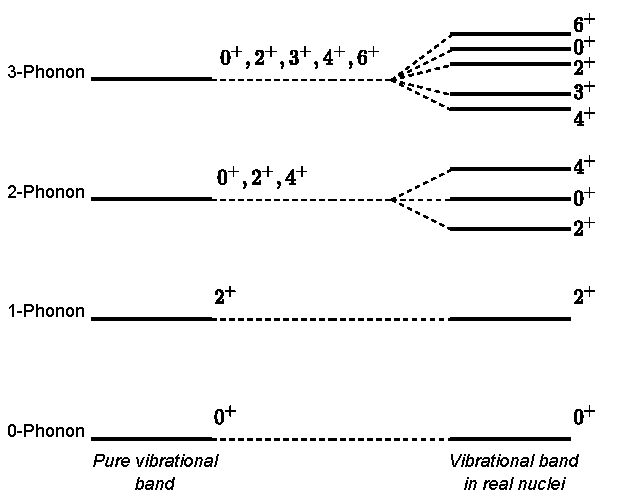
\includegraphics[width=0.99\textwidth]{Chapters/Figures/vibrational_states.pdf}
    \caption{Illustration of vibrational bands built as excitations of multiple phonons on a ground state. The left side reflects an ideal harmonic vibrator, with the degenerate spin states indicated for each level. Right side shows non-degenerate vibrational levels that exist in nuclei. Keep in mind that each phonon level is built as multiple excitations of a \emph{quadrupole phonon}.}
    \label{fig-vibrational-bands}
\end{figure}

% A general rule that is used to construct vibrational bands is related to the concept of \emph{symmetrized states}. Since the excited quanta are represented by phonons (identical bosons) having integer angular momentum (e.g., $\lambda=2$ for the quadrupole vibrations), the only spin states than can be observed in such spectra are the ones for which the final angular momenta couple to give symmetric combinations. This is the reason why in the energy state created by exciting the ground state $0^+$ with two phonons, only the states $0^+,2^+,4^+$ appear; the spin states $1^+$ and $3^+$ do not give symmetric combinations. A more generic method for determining which sequence of spins can be obtained by coupling angular momenta of vibrational phonons can be seen in Ref. \cite{ring2004nuclear}.

A quantity often used within the measurements of nuclear properties is the ratio between the second and the first excited states within a band. These ratios are usually denoted by $E(4^+)/E(2^+)$ (the state $4^+$ belongs to the triplet phonon state depicted in Fig. \ref{fig-vibrational-bands}), and the theoretical value for the vibrational model gives a value of $2$. However, some experimental results point out to a value close to $2.2$ for nuclei below $A=150$, and a constant value of $3.3$ for $150<A<190$ (refer to Fig. \ref{4state-2state-ratio}). It should be noted that for the latter case, the value of the ratio is specific to another kind of nucleonic motion: \emph{rotation}, which will be discussed in the following section.
Example of experimental \emph{vibrational bands} for several even-$A$ nuclei are shown in Fig. \ref{energy-levels-120Te-virbational-band}.
\begin{figure}
    \centering
    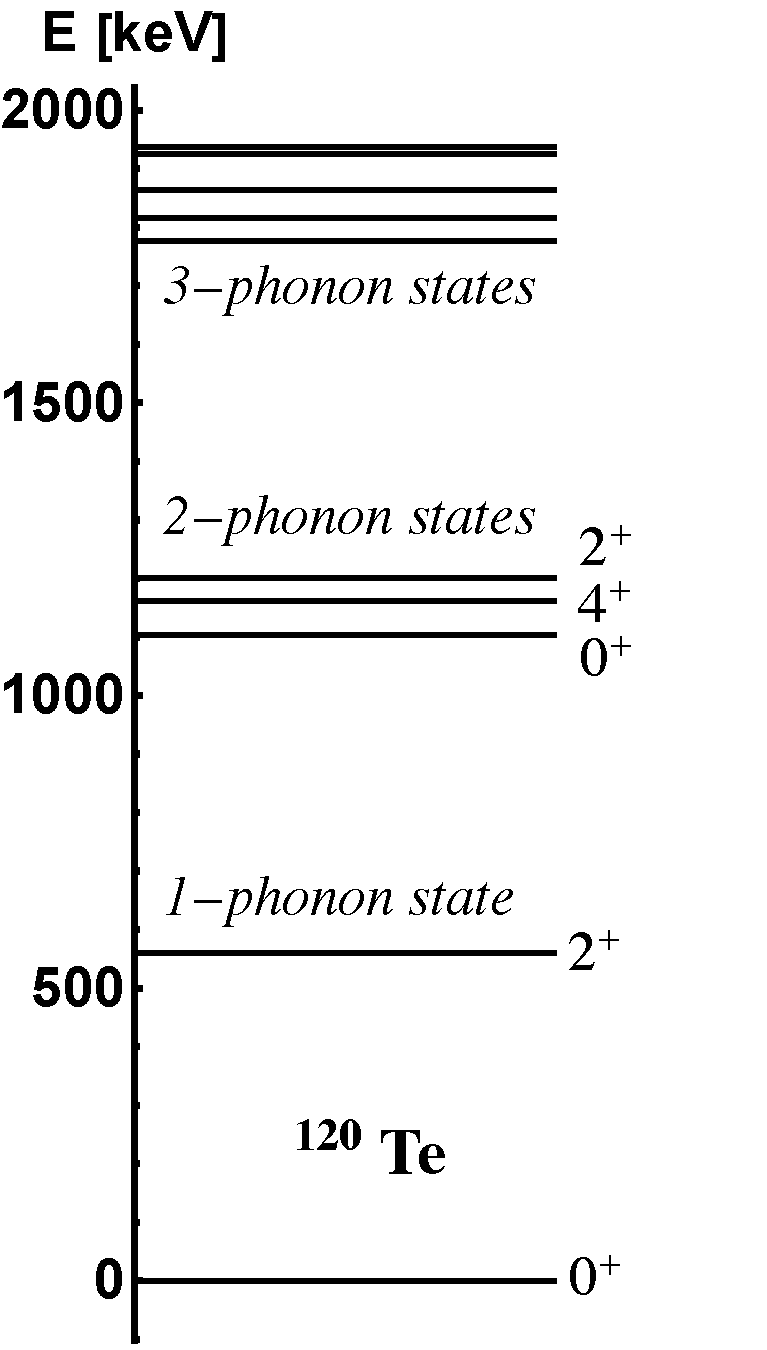
\includegraphics[width=0.32\textwidth]{Chapters/Figures/120Te_vib_experimental.pdf}
    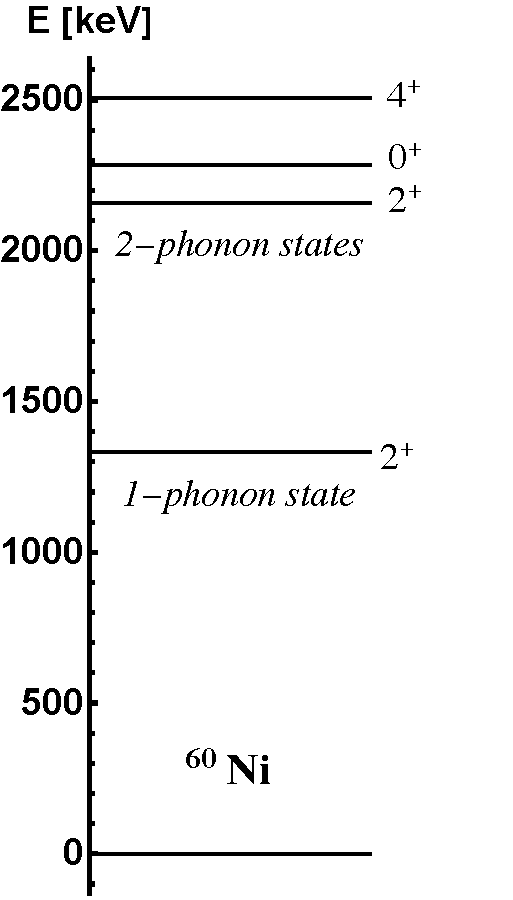
\includegraphics[width=0.32\textwidth]{Chapters/Figures/60Ni_vib_experimental.pdf}
    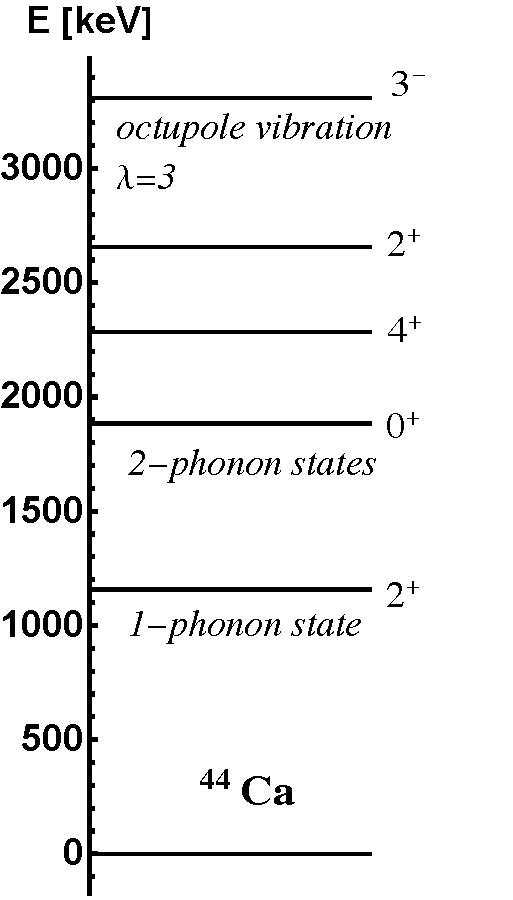
\includegraphics[width=0.32\textwidth]{Chapters/Figures/44Ca_vib_experimental.pdf}
    \caption{Vibrational bands in even-$A$ nuclei. \textbf{Left:} The experimental energy levels for $^{120}$Te. The triplet states that correspond to $\lambda=2$ can be seen, together with the quintuplet formed by adding three phonons to the $0^+$ ground state. Experimental data are taken from \cite{kitao2002nuclear}. \textbf{Middle:} The experimental data for $^{60}$Ni. For simplicity, only the first two phonon states are represented. Experimental data were taken from Ref. \cite{browne2013nuclear}. \textbf{Right}: The experimental data for a vibrational-like structure in $^{44}$Ca \cite{chen2011nuclear}. Note the highest energy level coming from the vibrational motion corresponding to an \emph{octupole} mode ($\lambda=3$).}
    \label{energy-levels-120Te-virbational-band}    
\end{figure}

There can also be vibrational bands in odd-$A$ nuclei. Indeed, if one considers the nucleus as a spherical even-even core plus an extra nucleon, the \emph{final} nuclear states are formed by coupling an individual $j$ orbit with the vibrational states of the core. An example is $^{63}$Cu, which has the ground state $3/2^{-}$. The g.s. for this nucleus is given by the last \emph{uncoupled} nucleon that occupies a shell. In fact, for this particular nucleus, it is the $2p_{3/2}$ proton that will give the final spin and parity of the nucleus. The vibrational spectrum is regarded as coupling the aforementioned proton with the $^{62}$Ni core. Indeed, by taking a $2^+$ vibrational phonon from the even-$A$ nucleus, then the (odd-proton + phonon) system can generate a sequence of energy states with angular momenta $I=1/2,\ 3/2,\ 5/2,\ 7/2$ and negative parity states. The energy levels depicted in Fig. \ref{energy-levels-63Cu-virbational-band} show the particle-core coupling effects on the vibrational structure in odd-mass nuclei.
\begin{figure}
    \centering
    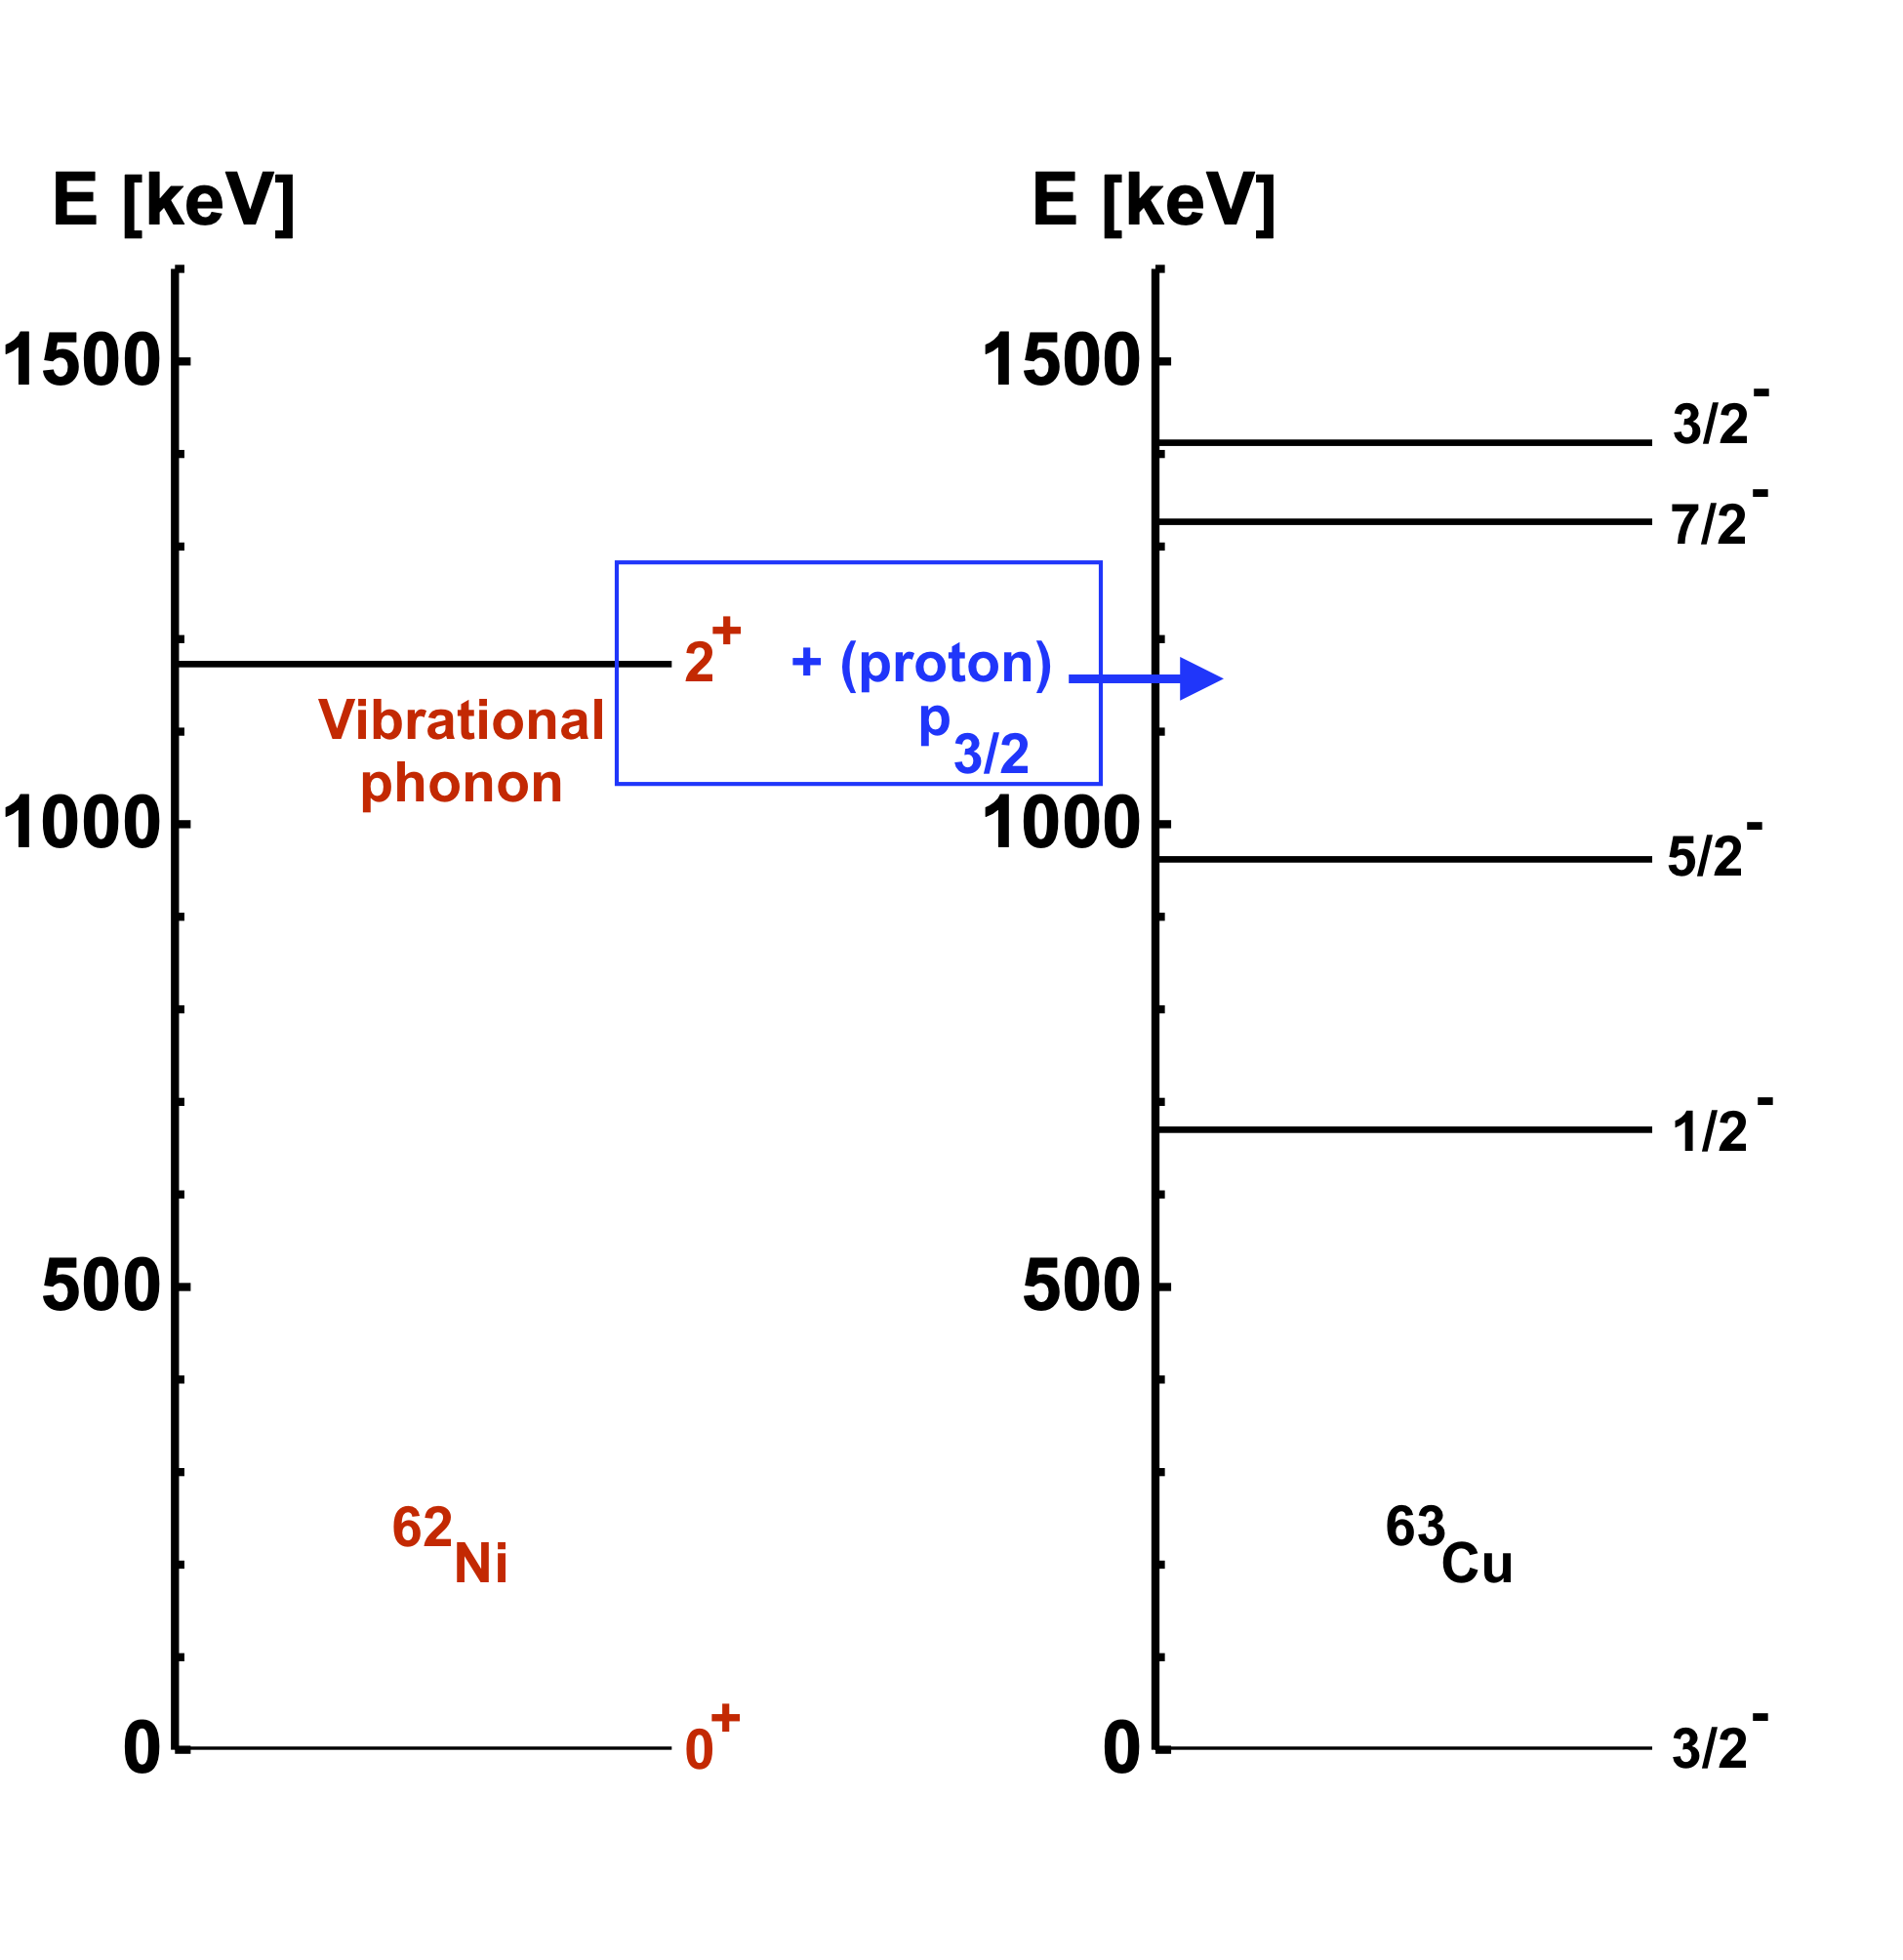
\includegraphics[width=0.8\textwidth]{Chapters/Figures/63Cu_vib_experimental.png}
    \caption{The experimental data of the vibrational states in $^{63}$Cu \cite{erjun2001nuclear}. The $2^+$ phonon state in $^{62}$Ni is also shown. The experimental data for $^{62}$Ni are taken from Ref. \cite{nichols2012nuclear}. The blue rectangle tries to emphasize that the quadruplet in $^{63}$Cu is formed by the coupling of the odd proton to the $2^+$ vibrational state from the neighboring nucleus.}
    \label{energy-levels-63Cu-virbational-band}
\end{figure}

Since the quadrupole vibrations carry an angular momentum of $\lambda=2$, there can be two types of vibrations in a deformed nucleus: one corresponding to $K=0$ and one for $K=2$. The $K=0$ vibrational motion is called $\beta$-vibration, and this induces a small fluctuations in the quadrupole deformation parameter, but it preserves the axial symmetry of the nucleus (the vibration is aligned with the deformation axis). The $K=2$ vibration is called the $\gamma$-vibration, which is responsible for fluctuations in the triaxiality parameter $\gamma$. A qualitative description for such an oscillation can be explained in terms of an american football \cite{krane1991introductory}: $\gamma$-vibrations consist of a simultaneous pushing and pulling of the ball on its sides, while the $\beta$ vibrations correspond to continuous pushing and pulling on the ends of the football. An illustration explaining the geometrical meaning of the $\beta$ and $\gamma$ vibrations in nuclei can be seen in Fig. \ref{rotation-vibration-geometrics}.
\begin{figure}
    \centering
    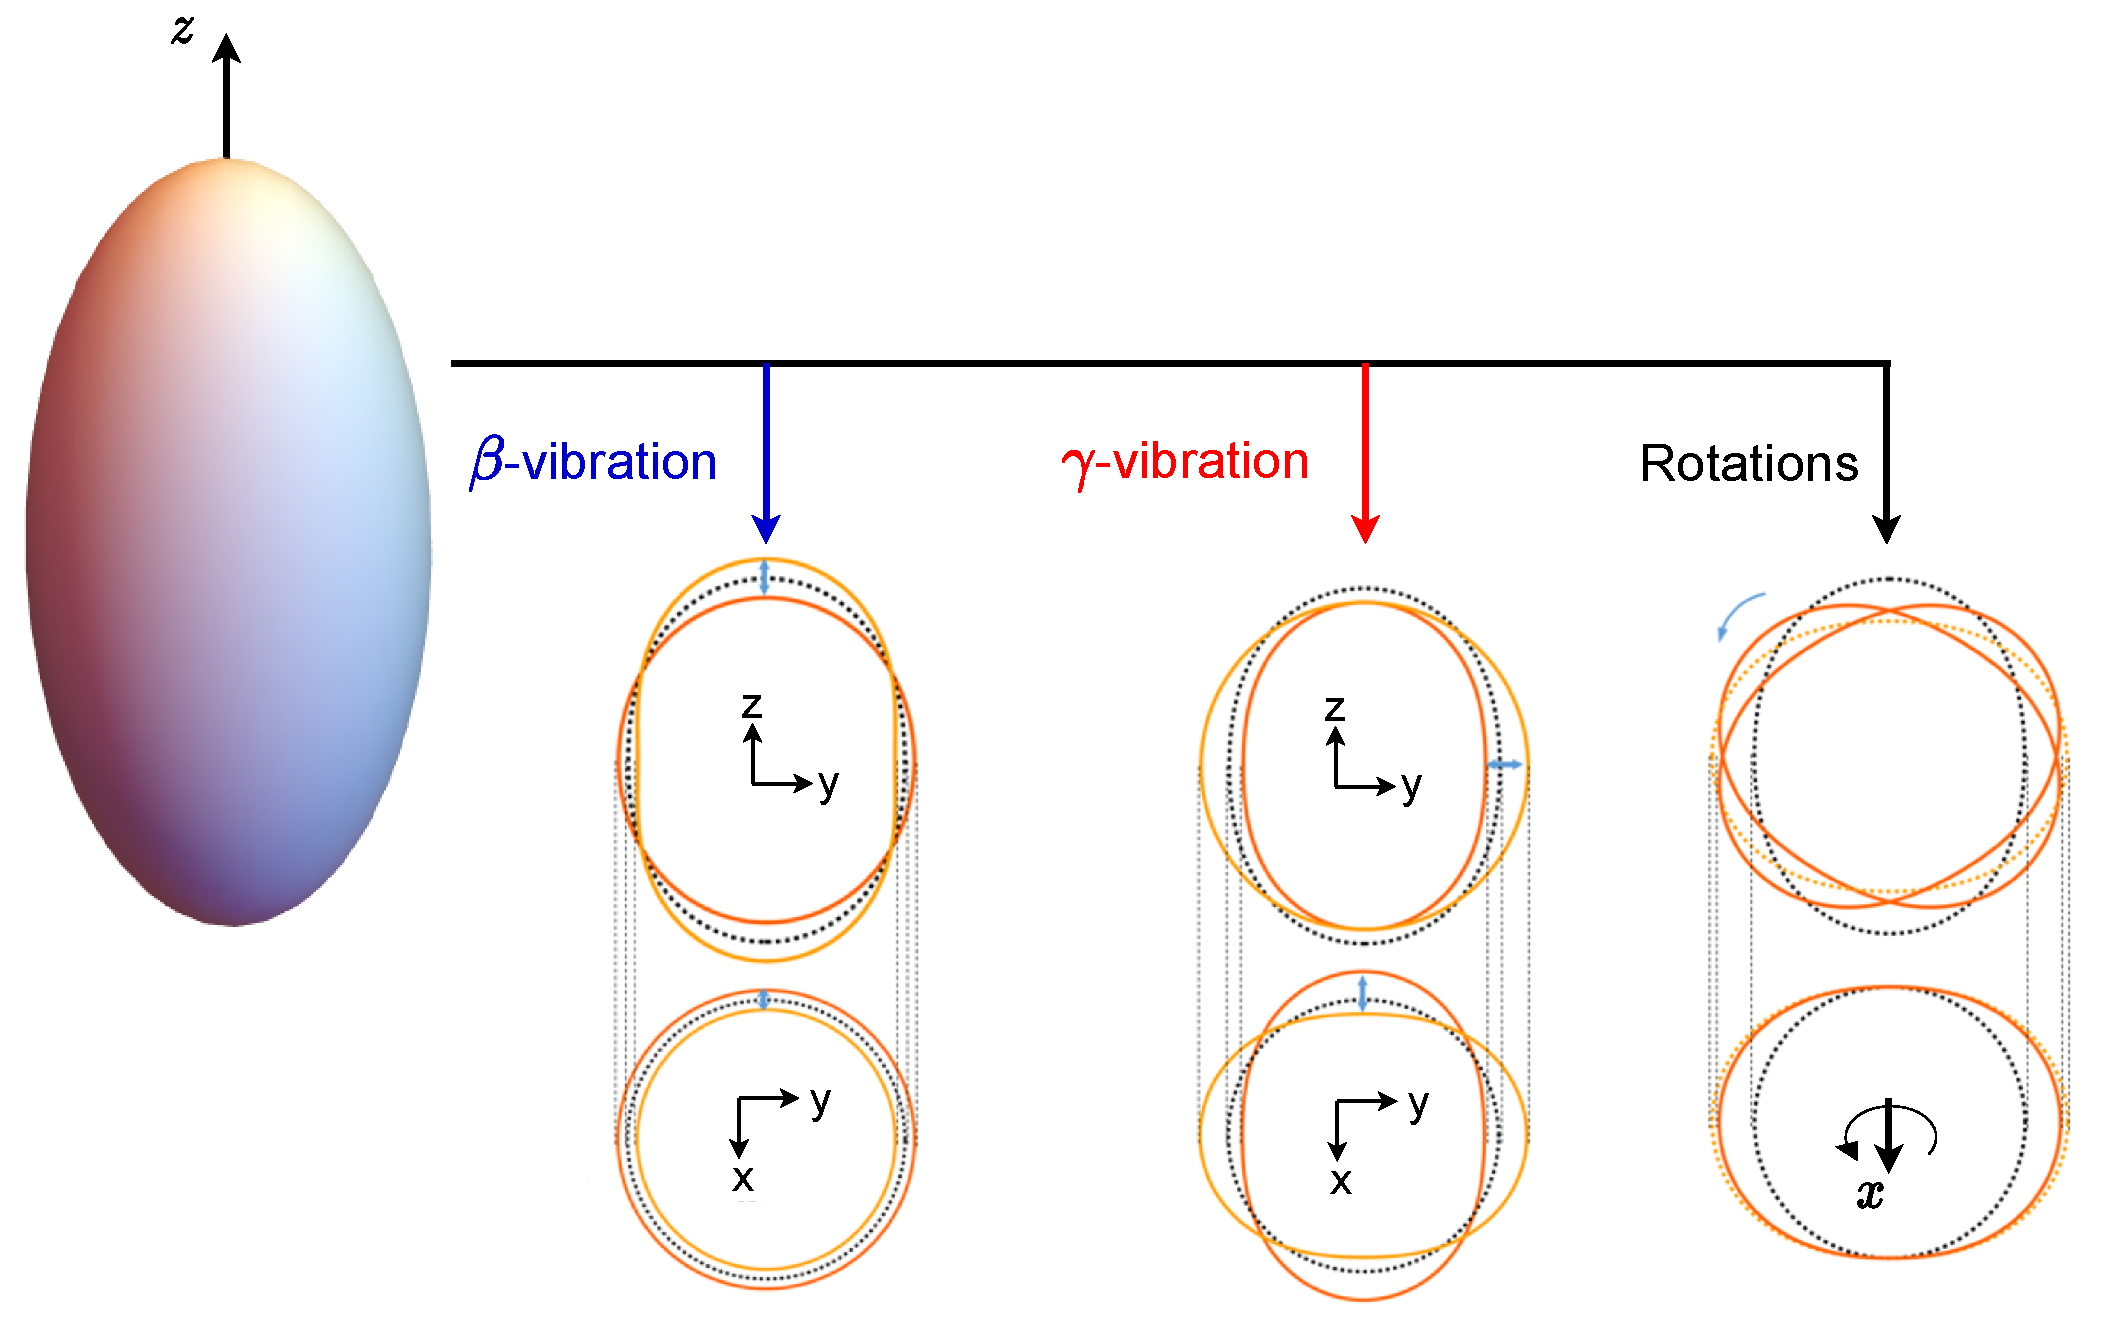
\includegraphics[width=0.99\textwidth]{Chapters/Figures/rotationsVibrations_Rotations.pdf}
    \caption{The $\beta$ and $\gamma$ vibrations occurring in nuclei. The initial nucleus in this example is of prolate type. Each mode of vibration is visualized from the side-view and top-view, respectively. This figure was inspired from Ref. \cite{li2022model}.}
    \label{rotation-vibration-geometrics}
\end{figure}

\section{Nuclear Rotation}

The rotational-kinetic term from $H_\text{coll}$ is called the \emph{rotational energy}, and its expression is given by \cite{corrigan1976exact}:
\begin{align}
    \hat{T}_\text{rot}=\frac{\hat{I}_1^2}{2\mathcal{I}_1}+\frac{\hat{I}_2^2}{2\mathcal{I}_2}+\frac{\hat{I}_3^2}{2\mathcal{I}_3}\ .
    \label{eq-rotational-energy-quantized}
\end{align}

The three operators that appear in Eq. \ref{eq-rotational-energy-quantized} are the projections of the total angular momentum $\mathbf{I}$ on the body-fixed axes (see Fig. \ref{rotational-coupling-schematic} for reference). Note that throughout the text, the angular momentum will be interchangeably represented with an arrow or by bold letters.

An important conclusion emerging from the work of Bohr and Mottelson \cite{bohr1954rotational} (also see discussion in Ref. \cite{greiner1996nuclear}) is that no rotations about the symmetry axis are possible for spherical nuclei or axially deformed nuclei. 
%Consequently, a prior deformation (e.g., of quadrupole type) and a rotating axis which does not coincide with the symmetry one are required for the appearance of rotational levels.
Indeed, every nucleus which contains energy states that are generated by the rotational motion has these bands due to the rotation about an axis that is different from the symmetry axis, and its shape is either axially-symmetric or axially-asymmetric \cite{hamamoto2016interplay}. In its motion, a nucleus can generate angular momentum in two ways:
\begin{itemize}
    \item \emph{collectively}: via combined rotations and vibrations of the nuclear droplet (the rotation + vibration spectrum of a nucleus will be shown in the next section)
    \item \emph{single-particle excitations}: unpaired nucleons can rearrange themselves in such a way that they account to the nuclear spin
\end{itemize}

The coupling of the droplet's rotational a.m. $\mathbf{R}$ with the single-particle angular momentum of a valence nucleon $\mathbf{j}$ can be seen in Fig. \ref{rotational-coupling-schematic}. Based on the expression of $T_\text{rot}$ from Eq. \ref{kinetic-rotational-energy-collective}, its quantized form given in Eq. \ref{eq-rotational-energy-quantized}, and the coupling scheme depicted in Fig. \ref{rotational-coupling-schematic}, it is possible to construct a Hamiltonian that corresponds to rotating nucleus with no valence particle. More precisely, the $\mathbf{j}$ term is neglected, such that only the pure collective motion of a nucleus is emphasized ($\mathbf{I}=\mathbf{R}$). The energy spectrum for an even-even nucleus is thus expressed as \cite{davydov1958rotational}:
% This approximation is however only valid for even-even nuclei and for the low-lying states \cite{bertulani2007nuclear,davydov1958rotational}:
% \begin{align}
%     H&=H_\text{rot}+H_\text{intr}=\sum_i\frac{\hbar^2}{2\mathcal{I}_i}R_i^2\ ,
% \end{align}
% where the second term $H_\text{intr}$ represents some effects coming from the internal structure of the rotator itself. However, most of the time these terms can be neglected, leading to a rather simple energy spectrum for the even-even nuclei:
\begin{align}
    E_\text{rot}(I)=\frac{\hbar^2}{2\mathcal{I}_\perp}I(I+1)\ .
    \label{eq-simple-rotor-spectrum}
\end{align}
\begin{figure}
    \centering
    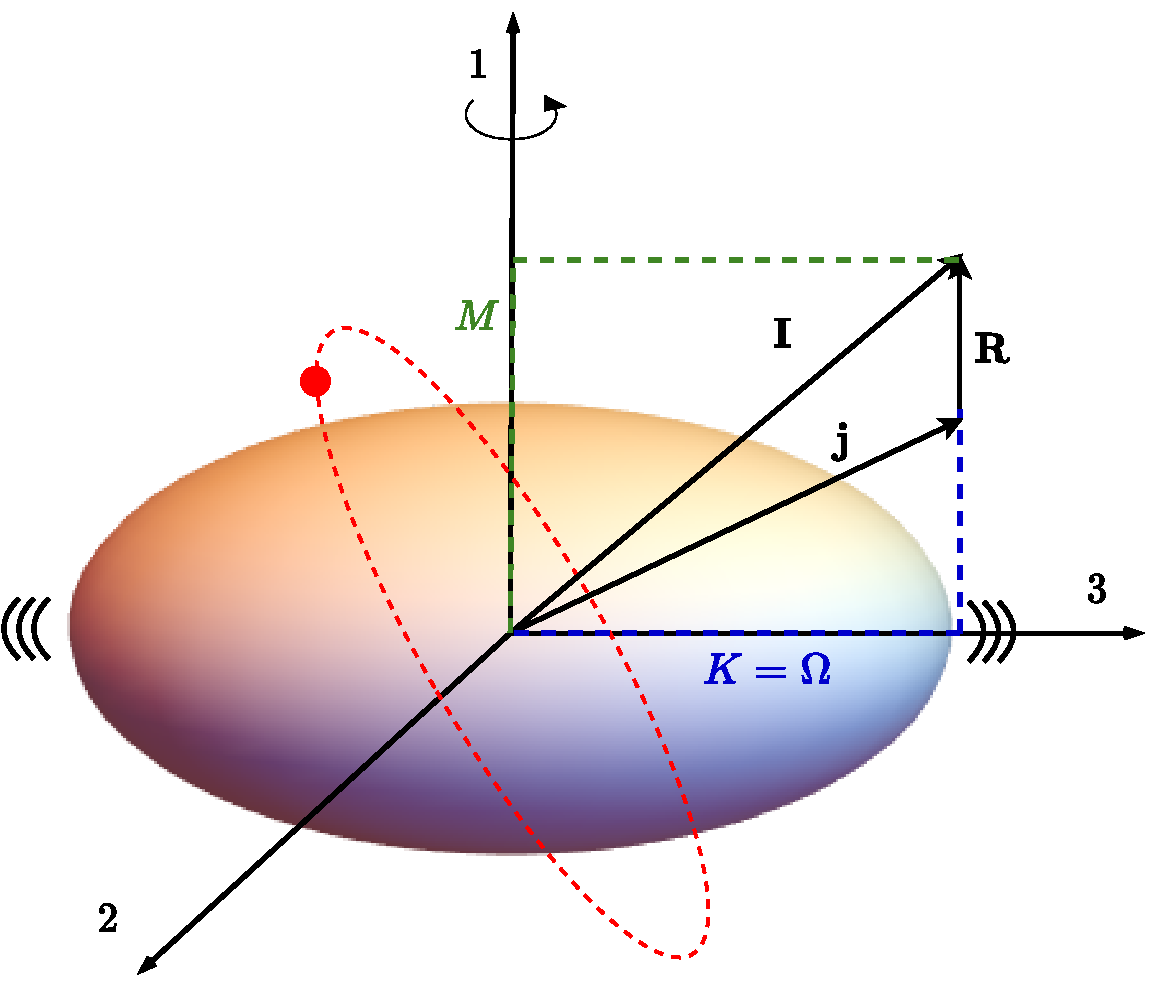
\includegraphics[scale=0.6]{Chapters/Figures/SCHEMATIC_COUPLING_ROTATIONAL.pdf}
    \caption{The coupling of the collective angular momentum with the angular momentum of a single-particle for an axially deformed nucleus that is rotating about an axis perpendicular to the deformation axis.}
    \label{rotational-coupling-schematic}
\end{figure}

In the above expression, $\mathcal{I}_\perp$ corresponds to an axis that is perpendicular to the symmetry axis (i.e., either $1$-axis or the $2$-axis) of the ellipsoid. In the case of axial symmetry both moments are equivalent, such that the general notation $\mathcal{I}_\perp$ is made. As an observation, since there is no single-particle contribution, the quantized angular momentum $I$ is equivalent to $R$. The spectrum defined by Eq. \ref{eq-simple-rotor-spectrum} leads to energy spacings $\propto I(I+1)$, which is also met in the molecular spectra. The ground-state will always be the state $0^+$, and due to the \emph{mirror symmetry} that is required for the wave-functions describing the even-even nuclei, every other excited state will be represented by an even value of the spin: $2^+,4^+,\dots$ \cite{ring2004nuclear}. The ratio $E(4^+)/E(2^+)$ for these bands is $3.33$. This is indeed the best signature for the rotational phenomena in nuclei, indicating a clear presence of deformation + rotational motion. In a previous work by the current team (Raduta et al. \cite{raduta2017semiclassical}), some spectra of even-even $^{158}$Er were studied, and agreement with the observed experimental data was impressive. The energy spectra obtained from Eq. \ref{eq-simple-rotor-spectrum} has a classical counterpart known within literature as the \emph{symmetric top}. Fig \ref{rotational-bands-even-even} shows some examples of rotational bands in even-$A$ nuclei.
\begin{figure}
    \centering
    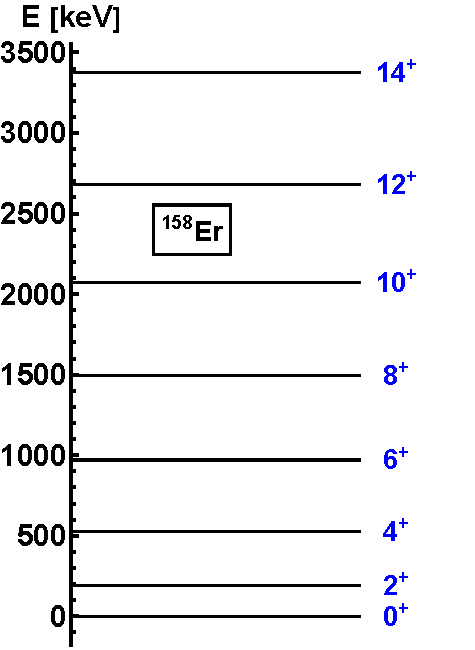
\includegraphics[scale=0.7]{Chapters/Figures/Er158-Rotational-Bands.pdf}
    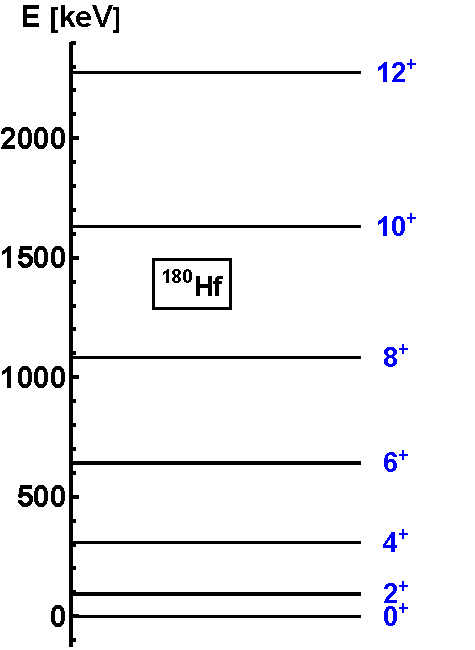
\includegraphics[scale=0.7]{Chapters/Figures/Hf180-Rotational-Bands.pdf}
    \caption{Experimental data showing the rotational bands in even-even nuclei. Note the spacing between the states that increases with $I$ via the rule from Eq. \ref{eq-simple-rotor-spectrum}. Experimental data are taken from Refs. \cite{nica2017nuclear,mccutchan2015nuclear}.}
    \label{rotational-bands-even-even}
\end{figure}

The spectra of a simple rigid rotator assumes that the projection $K$ of the total angular momentum for the ground-state of even-even nuclei is $K=0$. So the next step is to consider more general cases of nuclear rotation. There are two general cases of rotational bands that can occur, and both require the coupling scheme of a rotor with a valence nucleon, such that the angular momentum will be $\mathbf{I}=\mathbf{R}+\mathbf{j}$ (so both situations will correspond to odd-$A$ nuclei). The two situations are called \emph{Deformation aligned bands} and \emph{Rotation aligned bands} \cite{uwitonze2015assignment}. These are detailed in Appendix \ref{appendix:ral-dal-signature-scheme}.

\section{Superimposed Rotations and Vibrations}

Up until now, the collective rotations and vibrations were discussed separately. The small vibrations of the nuclear surface lead to band structures constructed via the quadrupole phonons carrying $\lambda=2$ units of angular momentum. The proper picture of a rotating deformed nucleus consists of a stable \emph{equilibrium shape} that is determined by $i)$ the \emph{rapid internal motion of the nucleons} within the nuclear potential and $ii)$ their entire distribution doing a \emph{slow rotation} having a negligible effect on the nuclear structure or on the individual nucleonic orbits.

Besides the two (separated) degrees of freedom for the nuclear system (i.e., collective rotation and vibrations), they can also be superimposed on each other. Starting from the expression of the \emph{Collective Bohr's Hamiltonian}, the spectrum can be described by the general Hamiltonian:
\begin{align}
    H_\text{coll}=T+V=T_\text{vib}+T_\text{rot}+V
\end{align}

A separation of the Hamiltonian terms in three main components will be made: one associated to the $\beta$-vibration, one for $\gamma$-vibrational mode, and the third term is the rotation of a rigid rotor characterized by a total spin $I$ and well-defined MOI. Following the separation, the spectrum will be \cite{ring2004nuclear,li2022model}:
\begin{align}
    E_{n_\beta n_\gamma IK}=\hbar\omega_\beta\left(n_\beta+\frac{1}{2}\right)+\hbar\omega_\gamma\left(n'_\gamma+\frac{1}{2}|K|\right)+\frac{\hbar^2}{2\mathcal{I}}\left[I(I+1)-K^2\right]\ .
    \label{collective-rotation-vibration-energy-spectrum}
\end{align}

Note the two harmonic-like solutions that make the vibrational mode present in the energy formula. The two `frequencies' are given in terms of the stiffness and inertia parameters.
\begin{align}
\omega_\beta=\sqrt{\frac{C_0}{B_2}}\ ,\ \omega_\gamma=\sqrt{\frac{C_2}{B_2}}\ ,   
\end{align}
and the two quantum numbers are as follows \cite{li2022model}: 
\begin{align}
    n_\beta&=0,1,\dots\ ,\\
    n'_\gamma&=2n_\gamma+1\ ,\ n_\gamma=0,1,\dots\ .
\end{align}
The allowed values for the quantum numbers are as \cite{li2022model}:
\begin{align}
    K&=0,2,4,\dots\ ,\nonumber\\
    I&=\begin{cases}
        K,K+1,K+2,\dots &\text{for} K\neq 0\\
        0,2,4,\dots &\text{for} K=0\\
    \end{cases}\ .
\end{align}

Consequently, the spectrum of a typical nucleus in which both vibration and rotation occur has a set of bands that are characterized by the quantum numbers $K,n_\beta,n_\gamma$. This collective spectrum is exemplified in Fig. \ref{collective-rotation-vibration-energy-levels}, and the main bands are:
\begin{enumerate}
    \item the ground-state band, having states with even $I$, where excitation energies are constructed from the rotor term
    \item the $\beta$ band, starting above the g.s. band with $\hbar\omega_\beta$ and containing only even spins
    \item the $\gamma$ band, corresponding to $K=2$ (as explained in a previous section). It is distinguished from the $\beta$ band because it starts with $2^+$ as first state and it contains both odd and even spins.
    \item the higher-level bands are the $n_\gamma=1$ and $K=4$ bands for $\gamma$-vibrational mode, and the $\beta$ band with $n_\beta=2$.
\end{enumerate}
\begin{figure}
    \centering
    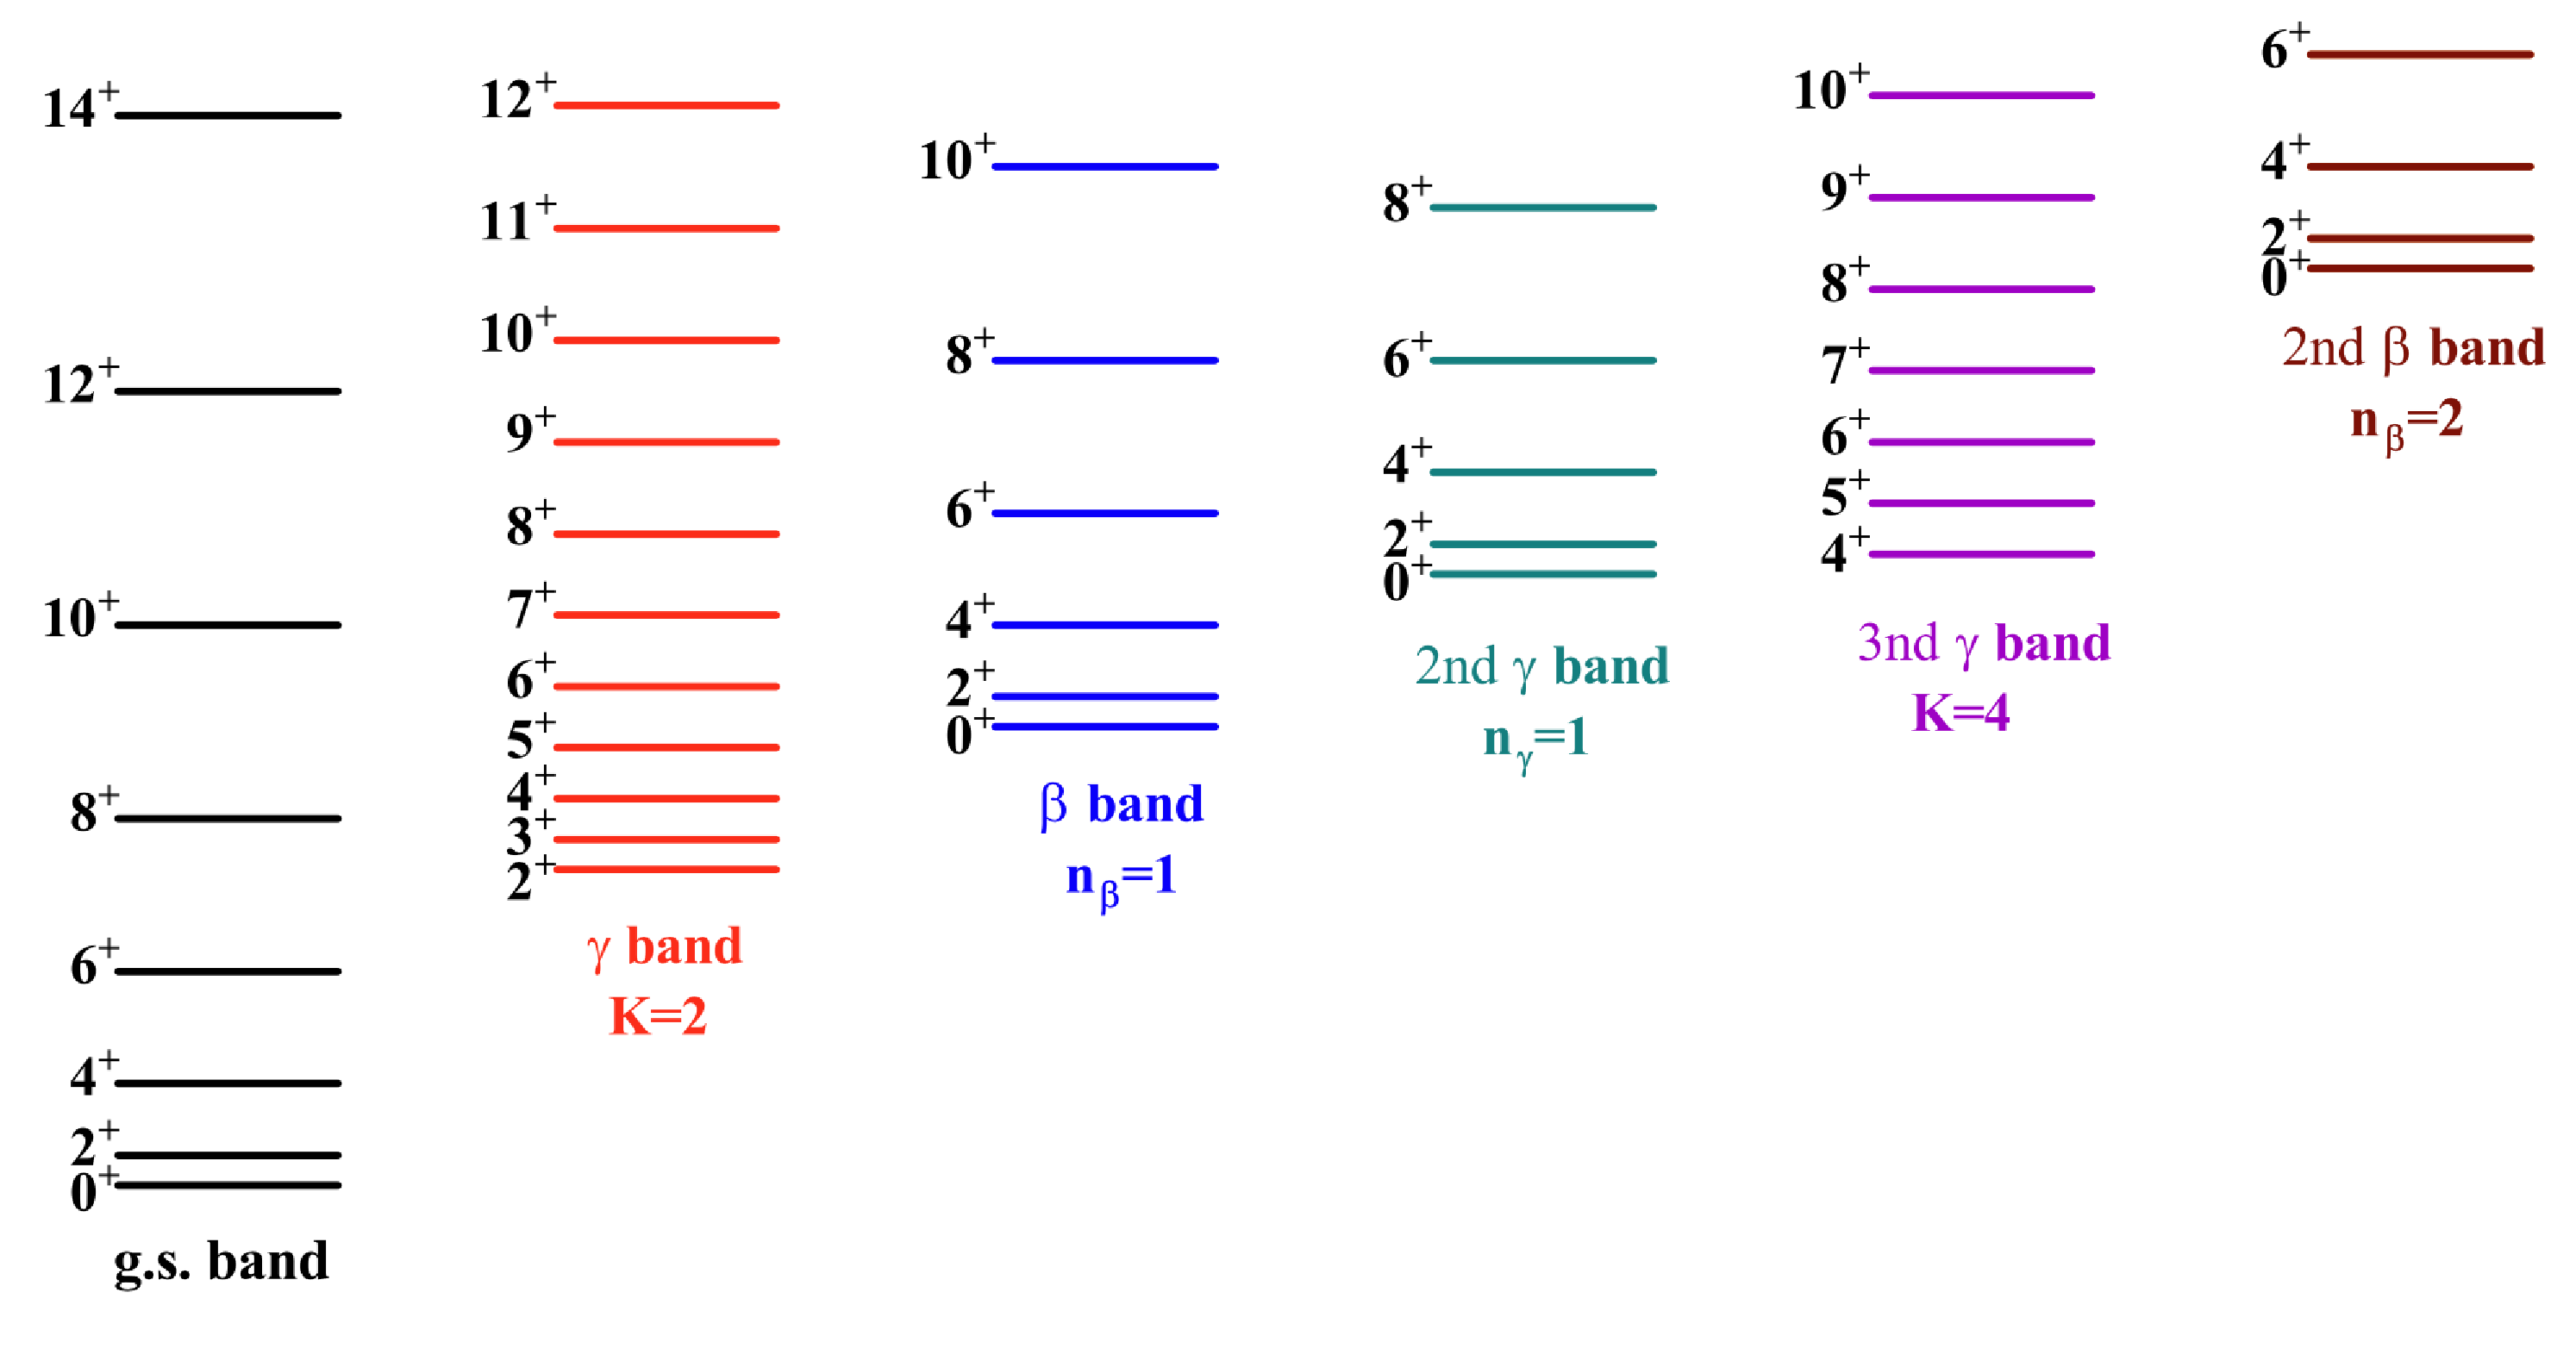
\includegraphics[width=0.99\textwidth]{Chapters/Figures/types_collective_bands.pdf}
    \caption{The energy spectrum specific to the Collective Model with \emph{Rotations + Vibration}. Each quantum number is also shown at the bottom of the bands. This figure is taken from Ref. \cite{li2022model}.}
    \label{collective-rotation-vibration-energy-levels}
\end{figure}

\section{Collective Quantities}
\label{c3-collective-quantities}

In this section, some important quantities that are strictly related to the collective nature of nuclei will be described. Indeed, one can understand nuclear deformation, energy spectra, and behavior of nuclei with respect to spin by studying quantities such as \emph{rotational frequencies}, \emph{moments of inertia}, \emph{quadrupole moments}, and so on. The comparison with experimental data for these quantities can help validate the theoretical assertions that are initially made, which represents a crucial test of any model.

\subsection{R - Energy Ratio}

As discussed before, the energy ratio between the first excited $4^+$ state to the first excited $2^+$ state is a very good test of rotational or vibrational spectra of nuclei. The evolution of this ratio across the mass number $A$ and a classification between \emph{vibrational} vs. \emph{rotational} character is made in Fig. \ref{4state-2state-ratio}.
\begin{figure}
    \centering
    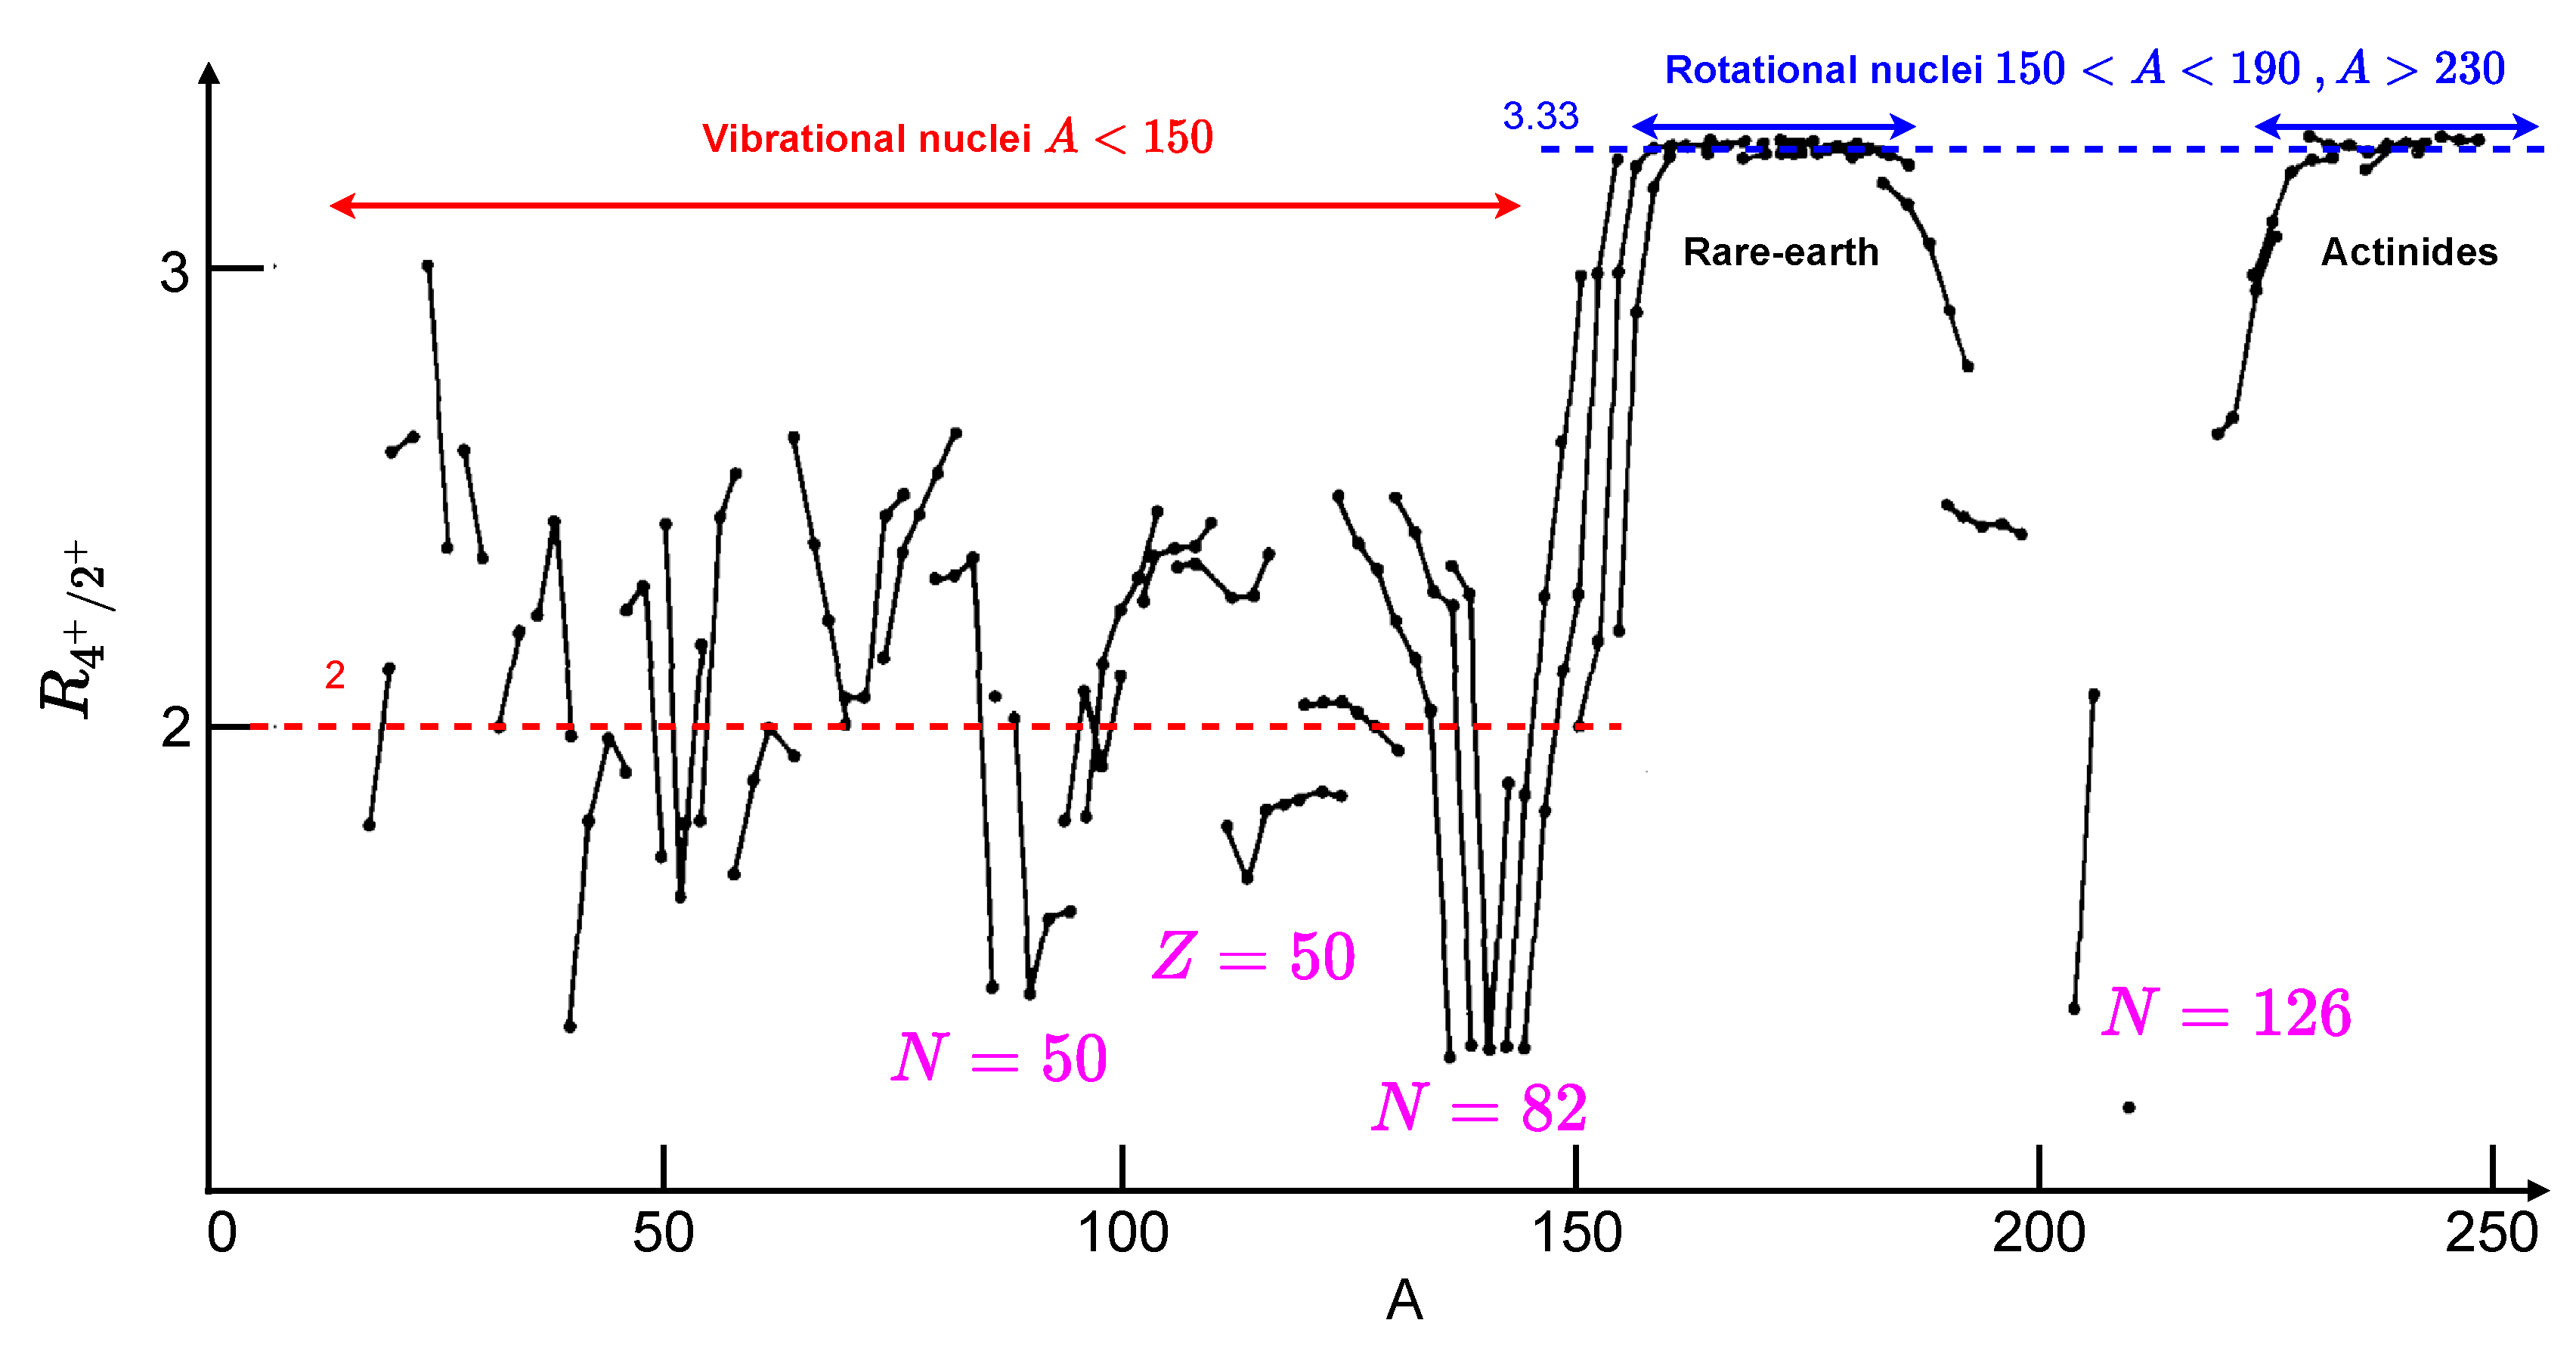
\includegraphics[width=0.99\textwidth]{Chapters/Figures/vibrations_rotations_E42-ratio.pdf}
    \caption{The experimental ratio $R_{4^+/2^+}$ in even-$Z$ and even-$N$ nuclei. Each line is connecting sequences of isotopes. Note the two important values for $R_{4^+/2^+}$, namely $2$ and $3.33$ given for a perfect vibrator and a pure rotator, respectively. Text with magenta color marks the magic numbers for $Z$ or $N$. This plot was inspired from Ref. \cite{casten2000nuclear}.}
    \label{4state-2state-ratio}
\end{figure}

\subsection{Rotational Frequencies}

In the classical limit the angular frequency:
\begin{align}
    \omega=l_\text{cls.}/\mathcal{I}\ ,
\end{align}
describes the kinetic energy of a rotating object. Indeed, $\omega$ is frequency of rotation around a particular direction, and its quadratic behavior gives the energy:
\begin{align}
    E=\frac{1}{2}\mathcal{I}\omega^2\ ,
\end{align}

The above expression can also be given in terms of the angular momentum $l_\text{cls.}$, such that the final energy becomes $E_\text{cls.}=l_\text{cls.}^2/(2\mathcal{I})$. Quantum mechanically, it was shown that $l^2$ is expressed as $\hat{l}^2_\text{quantum}=\hbar^2 l(l+1)$. Bengtsson et al. \cite{bengtsson1979quasiparticle} calculated the so-called \emph{Routhians} (single-particle energies within the rotating frame of reference), and they found a \emph {canonical} relation between the energies and rotational frequencies:
\begin{align}
    \omega=\frac{\text{d}E(I)}{\text{d}I_x}\ ,
    \label{rotational-frequency-canonical-definition}
\end{align}
where the term $I_x$ is called the \emph{aligned angular momentum}, and it usually denotes the experimental spin of every state minus a reference value \cite{harris1965higher}. The signature property discussed in Appendix \ref{appendix:ral-dal-signature-scheme} plays a pivotal role in determining $I_x(I)$, since the projection $K$ of the angular momentum onto the deformation axis must be taken into account:
\begin{align}
    I_x(I)=\sqrt{\left(I+\frac{1}{2}\right)^2-K^2}\ ,
    \label{aligned-angular-momentum}
\end{align}

In the case of $K=0$ bands, the aligned angular momentum reaches a simplified form $I_x^2=(I+\frac{1}{2})^2$. The value of $K$ is typically the band-head's angular momentum \cite{bengtsson1979quasiparticle,bengtsson1984signature}. Alternatively, for a sequence of states where $\Delta I=2\hbar$, the rotational frequency is usually calculated as:
\begin{align}
    \omega\equiv\hbar\omega_\text{rot}(I)=\frac{E_\gamma(I\to I-2)}{2}\ .
    \label{rotational-frequency-canonical}
\end{align}

% A more concise definition for the rotational frequency is related to the transition between two consecutive states $I+1\to I-1$ within a rotational band: a unique value of $\omega$ is attributed to the spin $I$, which is defined as a mean value of the two angular momenta from the corresponding transition. Such a construction will yield a set of discrete points $\omega(I)$, and one can obtain a `continuous' function $\omega(I)$ together with its inverse $I(\omega)$, thus making the term $I$ from Eq. \ref{aligned-angular-momentum} to be in fact $I(\omega)$.

The rotational frequency is used to represent many quantities that characterize collective motion and nuclear deformation. Representing the total or the aligned angular momenta as functions of $\omega$ can show wether multiple bands have the same nature. Moreover, representing the MOI as function of $\omega$ will also give an insight on the intrinsic structure of the nucleus. Another interesting feature that is present in high-spin spectra of nuclei is the so-called \emph{backbending} phenomena. This phenomenon appears due to the Coriolis effect: nucleons can suffer a de-pairing that makes their a.m. to align with the rotational axis, causing a sharp increase in the MOI \cite{ring2004nuclear,kvasil2004backbending}. These kind of effects are correlated to high deformation, increased rotation, and change in the nucleonic alignment.

\subsection{Moments of Inertia}

This is a crucial quantity that describes the degree of deformation and asymmetry of the nuclear shape (remember discussion from Chapter \ref{chapter-2}). It is possible to retrieve an \emph{experimental} value for the MOI by inferring the energy spacing between consecutive levels of a collective spectrum. A classification of types of MOI was done in Eq. \ref{eq-irrotational-rigid-mois}, where the MOI dependence on the deformation parameters and even the mass parameter $B_\lambda$ was shown. The most general expression for the MOI can be written as \cite{ahmad2021backbending}:
\begin{align}
    \mathcal{I}=\frac{\hbar^2}{2}\left(\frac{\text{d}E}{\text{d}J(J+1)}\right)^{-1}\ ,
\end{align}
where the classical angular momentum $J$ is related to its quantum equivalent via the correction $J=I+1/2$ (see Eq. \ref{aligned-angular-momentum}). Practically, the derivative can be expressed in terms of the aligned angular momentum $I_x$. Moreover, there are two types of MOI describing the characteristics of the rotational bands: the \emph{kinematical} and \emph{dynamical} moments of inertia. The kinematic MOI is given by \cite{wu1992relation}:
\begin{align}
    \mathcal{I}^{(1)}=\frac{\hbar I_x}{\omega}=\hbar^2 I_x\left(\frac{\text{d}E}{\text{d}I_x}\right)^{-1}\ ,
    \label{kinematic-moi-general}
\end{align}
% One can see why the aligned angular momentum is important, since its variation w.r.t. the energies lead to theoretical determinations of the kinematic MOI. From the observed intraband $E2$ transitions one can extract the (kinematic) moment of inertia via the rule:
% \begin{align}
%     \mathcal{I}^{(1)}(I-1)=\hbar^2\frac{2I-1}{E_\gamma(I,I-2)}\ ,
%     \label{kinematic-moi-energy-levels}
% \end{align}
% where $E_\gamma(I,I-2)$ represents the energy difference between two consecutive levels $E(I)$ and $E(I-2)$. The dependence on $I$ for this type of MOI makes its experimental determination to require some spin assignments to each state of the excited spectrum.
while the dynamic moment of inertia is expressed as \cite{wu1992relation}:
\begin{align}
    \mathcal{I}^{(2)}(I)=\hbar\frac{\text{d}I_x}{\text{d}\omega}=\hbar^2\left(\frac{\text{d}^2E}{\text{d}I_x^2}\right)^{-1}\ ,
    \label{dynamic-moi-general}
\end{align}
or, equivalently, as:
\begin{align}
    \mathcal{I}^{(2)}(I)=\hbar^2\frac{4}{\Delta E_\gamma(I)}=\hbar^2\frac{4}{E_\gamma(I+2,I)-E_\gamma(I,I-2)}\ .
    \label{dynamic-moi-energy-levels}
\end{align}

%Note that any calculations for the dynamical MOI does not require prior knowledge about the spin assignments. These two types of MOI are usually represented as function of the rotational frequency $\omega$. Since the total spin $I$ can be expressed as a function of rotational frequency, plotting the kinematic/dynamic MOI as function of angular momentum is also preferred. In the present work, these quantities are of high interest (graphical representations for different nuclei will be shown in a future chapter), their relative behavior will help characterize bands with similar nucleonic structure.

% An alternative description for these MOI can be done through the so-called $ab$ formula \cite{wu1992relation,wu1992spin}, where the energies corresponding to the rotational spectrum are parametrized as:
% \begin{align}
%     E(I)=a\left(\sqrt{1+bI(I+1)}-1\right)
%     \label{ab-formula}
% \end{align}

% Fitting the experimental data will produce a set of parameters $a$ and $b$ that will be used to get expressions for the kinematic and dynamic MOI:
% \begin{align}
%     \mathcal{I}^{(1)}=\mathcal{I}_0\left[1-\frac{(\hbar\omega)^2}{a^2b}\right]^{-1/2}\ ,\\
%     \mathcal{I}^{(2)}=\mathcal{I}_0\left[1-\frac{(\hbar\omega)^2}{a^2b}\right]^{-3/2}\ ,
% \end{align}
% where $\mathcal{I}_0$ is defined as the \emph{band-head} moment of inertia: $\mathcal{I}_0=\hbar^2/(ab)$. In fact, such an approach of determining the MOIs of several odd-$A$ nuclei will consist in a future work of the same team. 

As mentioned, the sharp or abrupt irregularities of the MOI with respect to the increase in rotational frequency is known as backbending. The Figs. \ref{fig-hfNuclei-mois} - \ref{fig-ErYbnuclei-mois} show experimental MOI as function of the squared rotational frequency.
\begin{figure}
    \centering
    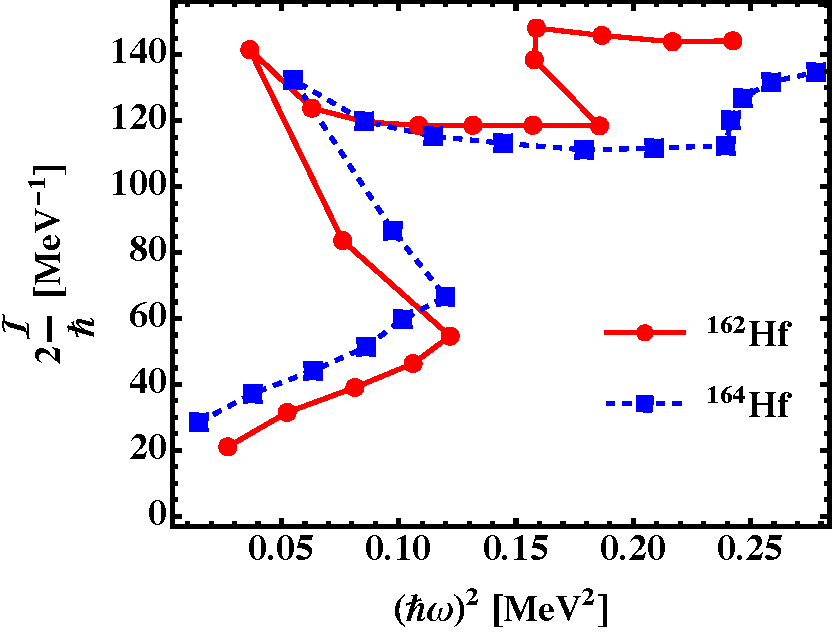
\includegraphics[scale=0.51]{Chapters/Figures/mois_Hf162-164.pdf}
    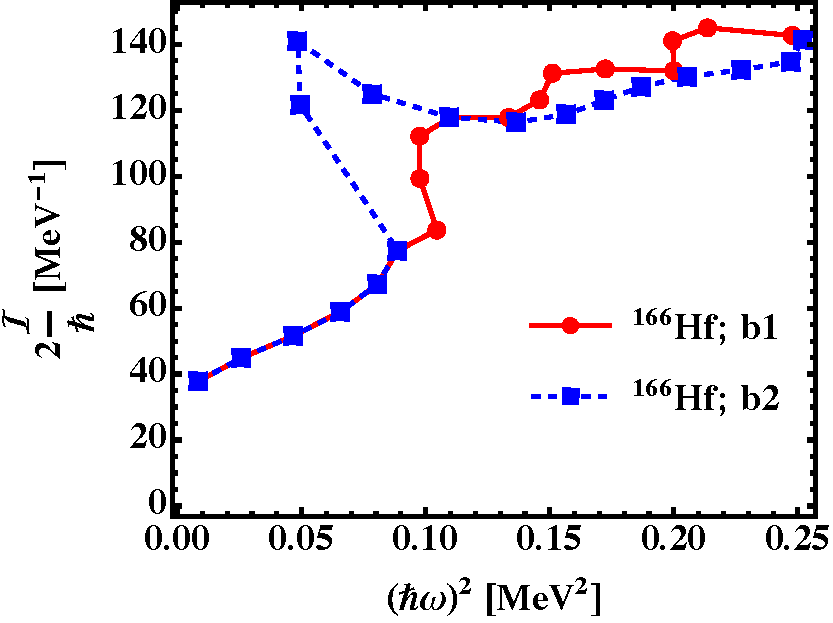
\includegraphics[scale=0.52]{Chapters/Figures/mois_Hf166.pdf}
    \caption{The moment of inertia as function of rotational frequencies for three even-even nuclei. \textbf{Left:} The MOI for $^{162,164}$Hf nuclei, with their corresponding rotational ground-state bands. \textbf{Right:} The MOI for the first two rotational bands in $^{166}$Hf. Experimental data for these two nuclei are taken from Ahmad et al. \cite{ahmad2021backbending}.}
    \label{fig-hfNuclei-mois}
\end{figure}
\begin{figure}
    \centering
    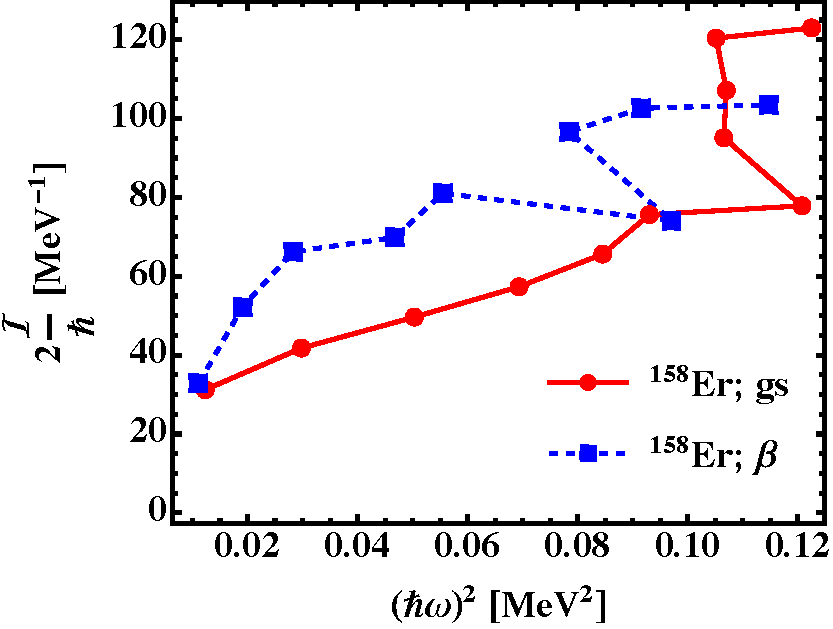
\includegraphics[scale=0.5]{Chapters/Figures/mois_Er158.pdf}
    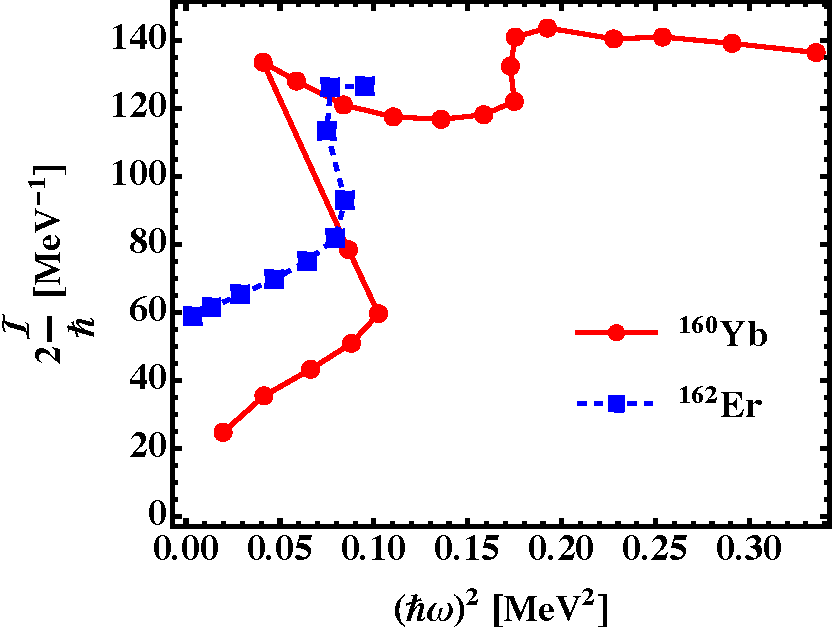
\includegraphics[scale=0.5]{Chapters/Figures/mois_Yb160Er182.pdf}
    \caption{\textbf{Left:} The MOI for $^{158}$Er nucleus, with the ground-state band $K^\pi=0^+$ and the $\beta$-vibrational band with the same quantum numbers. Experimental data are taken from \cite{nica2017nuclear}. \textbf{Right:} The MOI for $^{160}$Yb compared with $^{162}$Er. Experimental data are taken from \cite{nica2021nuclear} ($A=158$) and \cite{reich2007nuclear} ($A=162$).}
    \label{fig-ErYbnuclei-mois}
\end{figure}

Indeed, by looking at the evolution of $\mathcal{I}$ from Figs. \ref{fig-hfNuclei-mois} - \ref{fig-ErYbnuclei-mois}, some sharp increases are noted. These are usually attributed to the centrifugal stretching in the rotational model \cite{davydov1960rotation}. Moreover, the constant increase in $\mathcal{I}$ is considered to occur due to the slow and constant quenching of the pairing correlations between nucleons \cite{mottelson1960effect}. The abrupt changes are explained as rapid phase transitions of the nucleonic matter \cite{krumlinde1974effect} exclusively due to the Coriolis Anti-Pairing effect. On the other hand, backbending can also be explained via the band-crossing of two intersecting bands having different moments of inertia. Certainly, the \emph{non-crossing} effect (see Appendix \ref{appendix:two-state}) makes the bands approach each other as much as the interaction strength allows \cite{ring2004nuclear}. 
%Nevertheless, it is clear that the theoretical investigations point out the reduction of pairing correlations, which will affect the MOI at low spin. Finally, the alignment of nucleons will eventually cause backbending \cite{Stephens1974BackbendingAR,Stephens1972CoriolisEI}. 

% The band crossing is shown in Fig. \ref{bands-crossing-backbending}. This phenomenon starts from the idea of two bands with different moments of inertia: if one analyzes the plot of the energies w.r.t. the angular momentum $I$, at one point (a \emph{critical value} for $I$), the second band would intersect the first one, crossing it. But such a thing is forbidden, so there will be a change in behavior for the parabolas (left side plot from Fig. \ref{bands-crossing-backbending}), causing a simultaneous increase in total angular momentum and decrease in rotational frequency. This change in behavior is superimposed with the change in structure of the bands themselves, making the sharp transition possible. For small interaction strength between the two bands, the backbending will be quite `strong', while for large values the transition region is very broad, making the backbending non-occurring.
% \begin{figure}
%     \centering
%     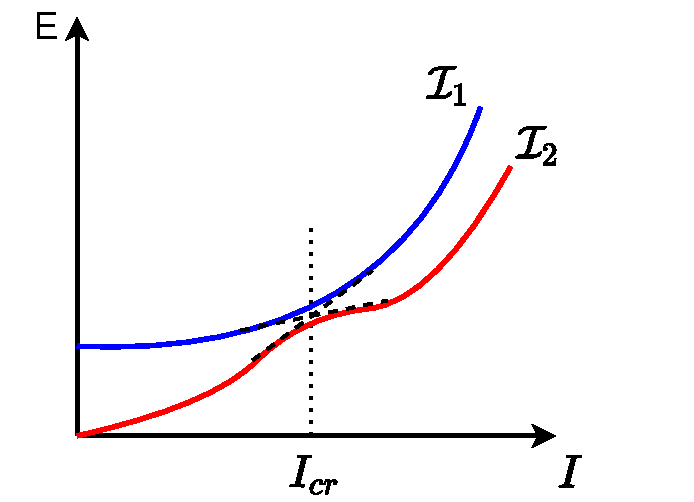
\includegraphics[scale=0.56]{Chapters/Figures/backbending_crossing_1.pdf}
%     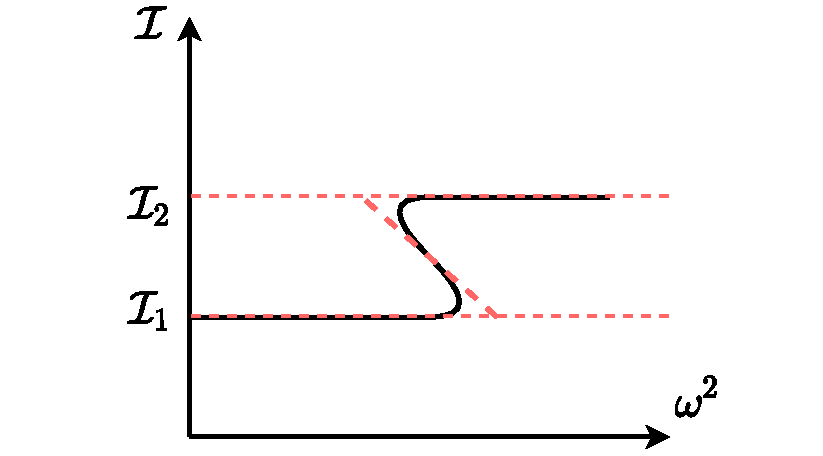
\includegraphics[scale=0.56]{Chapters/Figures/backbending_crossing_2.pdf}
%     \caption{An illustrative example with two bands that are interacting with each other, leading to backbending. This sketch was inspired from the work of Ring et al. \cite{ring2004nuclear}.}
%     \label{bands-crossing-backbending}
% \end{figure}

Usually, the graphical representations of the MOI (kinematic or dynamic) as functions of $\omega$ (or, equivalently, $I$) are useful when comparing multiple spectra in the same nucleus. Based on their behavior w.r.t. rotational frequency or spin, one can determine if the bands belong to the same intrinsic structure.
%For example, after spin and parity assignments of each energy state within the collective spectra of the odd-$A$ nucleus $^{163}$Lu, it is of interest to see how many sequences have \emph{normal deformation}, which single-particle + core couplings are preferred, if the bands have enhanced (strong) deformation, and so on. In the following chapters, a detailed overview with the evolution of the kinematic and dynamic MOI as a function of rotational frequencies for odd-$A$ around $A\approx 160$ nuclei will be made, since it plays a major role in the study of highly deformed nuclei. 
%The experimental data concerning $^{163}$Lu isotope allows one to check the experimental rotational frequencies $\hbar\omega(I)$, the \emph{alignment} $I_x$, and the two types of MOI which were discussed. These calculations are shown in Figs.
% A discussion about the backbending effect needs to be made, since it strictly connects to the paragraph just discussed above. Actually, within the region $10\sim20$ units of angular momentum this strange effect is observed, especially in the ground-state band (i.e., the \emph{yrast} band). The yrast line corresponds to the set of lowest energies for a given set of spin states \cite{bohr1954rotational}. In the work of Mariscotti el al. \cite{Mariscotti1969PhenomenologicalAO}, it was shown that for the lowest two orders, the moments of inertia can be approximated as $\mathcal{I}=\mathcal{I}_0+\mathcal{I}_1\omega^2$.

\subsection{Electric Quadrupole Moment}
\label{intro-EM-chapter3}

An important indicator of nuclear deformation is the \emph{electric quadrupole moment} \cite{hamamoto2016interplay}, which measures the `departure' of the nuclear shape away from spherical symmetry (through elongation and asymmetry). The most general expression of the intrinsic quadrupole moment for a rotating nucleus is given in terms of its \emph{charge density distribution} \cite{casten2000nuclear}:
\begin{align}
    Q_0=\int(3z^2-r^2)\rho(r)_\text{charge}\text{d}v\ .
    \label{general-quadrupole-moment-Q0-charge}
\end{align}

This shows how the nuclear charge distribution inside the nucleus plays a pivotal role in determining the nuclear deformation. A relationship between the deformation parameter $\beta$ and the quadrupole moment itself can be approximated (in second order of $\beta$) as \cite{krane1991introductory}:
\begin{align}
    Q_0=\frac{3}{\sqrt{5\pi}}R^2Z\beta(1+0.16\beta)\ ,
    \label{quadrupole-moment-Q0}
\end{align}
where $R$ is given as $R=R_0A^{1/3}$ and $R_0=1.2\ \text{fm}$. For values of $\beta$ that correspond to \emph{strongly deformed} nuclei (i.e., $\beta\sim 0.3$), higher order terms are not necessary. According to the discussion concerning the nuclear shapes, $\beta$ describes the eccentricity of the deformed ellipsoid (albeit prolate or oblate). The difference between a prolate and oblate ellipsoid is that for prolate (oblate) case there is an \emph{extension} in one (two) direction and a \emph{squeezing} in the other two (one). Depending on the value of $\beta$, the quadrupole moments for nuclei will be positive (indicating a prolate deformation) or negative (giving an oblate deformation). The experimental values of $\beta_2$ for rare-earth nuclei are shown in Fig. \ref{fig-quadrupole-beta-nuclides}. Note that for $\beta_2$ the subscript `2' will be used or dismissed freely throughout this work, but it will signify the same quantity. 
\begin{figure}
    \centering
    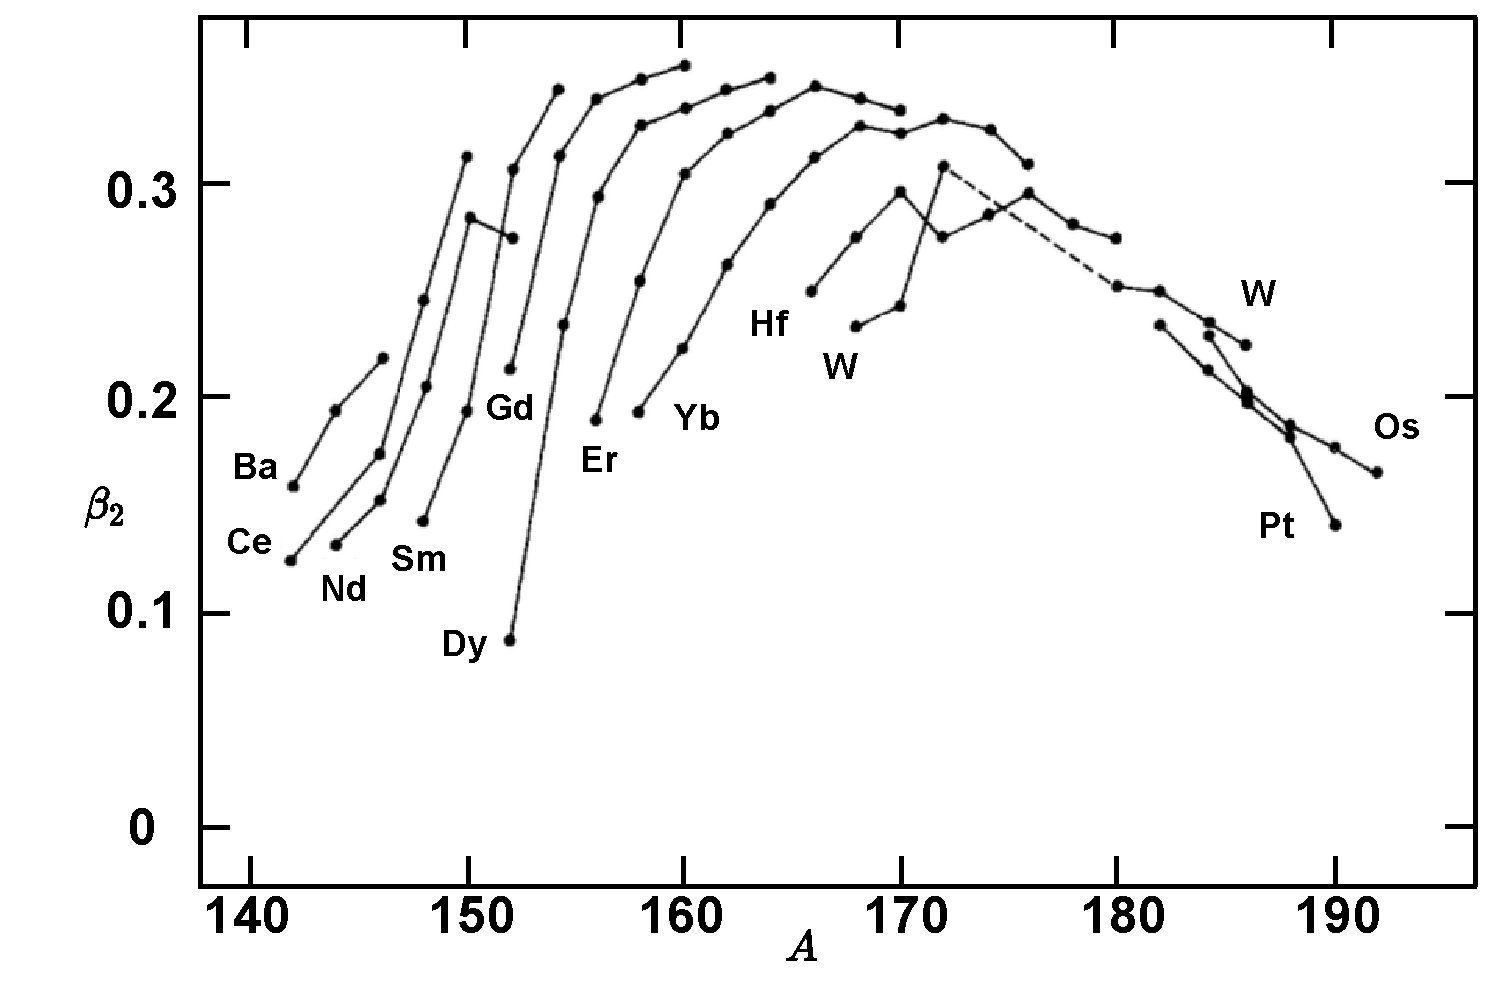
\includegraphics[width=0.99\textwidth]{Chapters/Figures/quadrupole_Deformation_rareEarth.pdf}
    \caption{The quadrupole deformation parameter $\beta_2$ as a function of the mass number $A$ for a few isotopes in the rare-earth region. These values were determined from the experimental transition probabilities $0^+\to 2^+$. The figure is reproduced from Ref. \cite{casten2000nuclear}.}
    \label{fig-quadrupole-beta-nuclides}
\end{figure}

In order to understand the behavior of $\beta_2$ shown in Fig. \ref{fig-quadrupole-beta-nuclides}, some shell-model considerations need to be taken into account. Firstly, when deformation kicks in, the individual $j$ orbits within a major shell are nearly empty, resulting in positive values for the quadrupole moments of the nucleons from these orbits. With increasing deformation, large and positive values $Q(\beta)$ are present. Furthermore, as the shells start to fill, contributions from individual $j$ orbits to the total quadrupole moment will accumulate, making its value to decrease, vanish, and eventually becoming negative near the shell closure \cite{casten2000nuclear}. %(see inset 3 in Fig. 5.4 from \cite{casten2000nuclear}).

The \emph{observed} quadrupole moment (also known as \emph{spectroscopic} or \emph{measured}) can be obtained via a transformation to the laboratory frame applied to $Q_0$, meaning that the spectroscopic quadrupole moment has the result \cite{casten2000nuclear}:
\begin{align}
    Q=\left[\frac{3K^2-I(I+1)}{(I+1)(2I+3)}\right]Q_0\ ,
    \label{quadrupole-moment-spectro}
\end{align}
where the quantum number $K$ is the projection of $I$ onto the symmetry (deformation) axis. The dependence of $Q$ on both $K$ and $I$ emphasizes the fact that the observed shape of a rotating nucleus is not equivalent to the shape in the intrinsic frame of reference. Consider the case of a prolate nucleus rotating about an axis that is perpendicular to the symmetry axis. Then the \emph{averaged} density distribution of the nuclear matter will look more like an oblate shape (see Fig. \ref{fig-averaged-prolate-density}). As a result, when the intrinsic quadrupole moment is positive, the observed one will have a negative value, resulting in the $I(I+1)>3K^2$ condition from Eq. \ref{quadrupole-moment-spectro}.
\begin{figure}
    \centering
    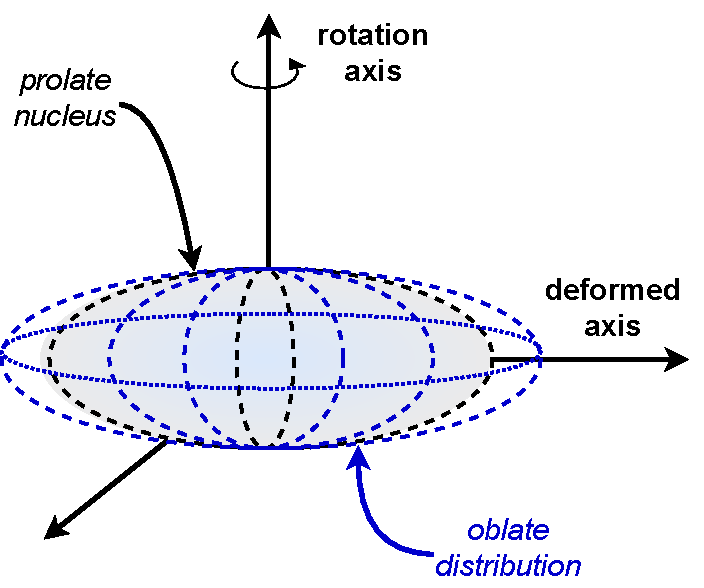
\includegraphics[scale=0.7]{Chapters/Figures/averaged_nuclearMatter_prolate.pdf}
    \caption{The average flattened (oblate) density distribution generated by the rotation of a prolate nucleus. As the `initial' prolate nucleus with its nuclear density (represented by the gray ellipse with dashed borders) being distributed along the deformed axis exhibits rotation, the rotated shape will generate an averaged oblate disk along the rotational axis (represented by the blue). This is why the observed quadrupole moment $Q$ will have a negative sign if $Q_0>0$.}
    \label{fig-averaged-prolate-density}
\end{figure}

Another important quantity used as a `test' for collectivity and deformation is the \emph{reduced electric quadrupole transition probability}, or $B(E2)$. This transition probability can be given in terms of the quadrupole moment introduced in Eq. \ref{general-quadrupole-moment-Q0-charge} through the following form \cite{bohr1998nuclear}:
\begin{align}
    B(E2;\ I_i\to I_f)=\frac{5}{16\pi}e^2Q_0^2\bra{I_iK20}\ket{I_fK}^2\ ,
    \label{reduced-E2-clebsch-gordan}
\end{align}
where the squared factor $\bra{I_iK20}\ket{I_fK}^2$ is the Clebsch-Gordan coefficient, also written as $\bra{I_iK20}\ket{I_fK}\equiv C^{I_i2I_f}_{K0K}$. In the case of $0^+\to 2^+$ transition, the reduced probability will be given by \cite{casten2000nuclear}:
\begin{align}
    B(E2;\ 0^+\to 2^+)=\frac{5}{16\pi}e^2Q_0^2\ .
    \label{reduced-E2-0Plus-2Plus-Transition}
\end{align}

The transition probability provided in Eq. \ref{reduced-E2-clebsch-gordan} is in fact a special case that can be applied to nuclei possessing \emph{axial symmetry}. This is because the involved transitions are not affected by a change of the projection $K$.
%A more general treatment of $B(E2)$ also requires prior knowledge of the so-called \emph{electric quadrupole transition operator}, which are not adopted here yet. This will be properly employed in a future chapter when discussing the transition probabilities in several odd-mass nuclei. 
From the quadratic dependence of the intrinsic quadrupole moment on $\beta$, high values (e.g. $\beta\approx 0.3$) will lead to $B(E2)$ that are one or even two orders of magnitude higher than those specific to nearly spherical nuclei $\beta_\text{sph}\approx 0.05$. Usually in nuclei, the valence nucleons are causing some core polarizations, which will affect the `final' structure of the electric quadrupole moment. For example, in an odd-$Z$ and even-$N$ nucleus, the total quadrupole moment $Q$ (also referred to as \emph{single-particle quadrupole moment} $Q_\text{s.p.}$) is given by the following expression \cite{bertulani2007nuclear}:
\begin{align}
    Q=-\langle r^2\rangle\frac{2j-1}{2j+2}\frac{e_\text{eff}}{e}\equiv Q_\text{s.p.}\ ,
    \label{single-particle-quadrupole-moment}
\end{align}
where $e_\text{eff}$ represents the \emph{effective charge} of the nucleus \cite{heyde1994nuclear}. The mean squared radius corresponds to the radial function of the particle within that $j$ orbital. 
%Stable nuclear deformation will require that the nuclear energy should be minimal. This can be achieved either if the overlap of the core with the valence particle is maximal, which for  a particle+core interaction will produce an oblate polarization, driving the nucleus to a final oblate deformed state. The opposite is true for the hole+core coupling (see discussion made in \cite{neugart2006nuclear}).
An interesting characteristic emerging from Eq. \ref{single-particle-quadrupole-moment} is that the odd-$A$ nuclei having $I=1/2$ will give a vanishing quadrupole moment $Q$. Although this situation concerns the measured (i.e., observed) moment, the odd-$A$ nucleus with $I=1/2$ does not necessarily imply that the system has no quadrupole moment. In fact, according to Eq. \ref{quadrupole-moment-spectro}, the spectroscopic moment is expressed in terms of the intrinsic component $Q_0$, so it is possible to have a vanishing $Q$ but $Q_0$ different from zero. The same circumstance is also met for the case of even-even nuclei.

The experimental data from Fig. \ref{experimental-Q-odd-nuclei} show the magnitude of $Q$ that would correspond to the value given by Eq. \ref{single-particle-quadrupole-moment}. One can see sharp increases with the nucleonic number for some nuclei (e.g., $^{167}$Er or $^{175}$Lu) but also very strong decreases to negative values (e.g., $^{123}$Sn). These alternations between positive (prolate) and negative (oblate) $Q$ values are also located near the magic numbers. Moreover, when the odd-particle is a neutron, the nucleus still exhibits a quadrupole moment that is different from zero, meaning that to some extent, the last nucleon is not the sole player regarding the quantitative behavior of $Q$.
\begin{figure}
    \centering
    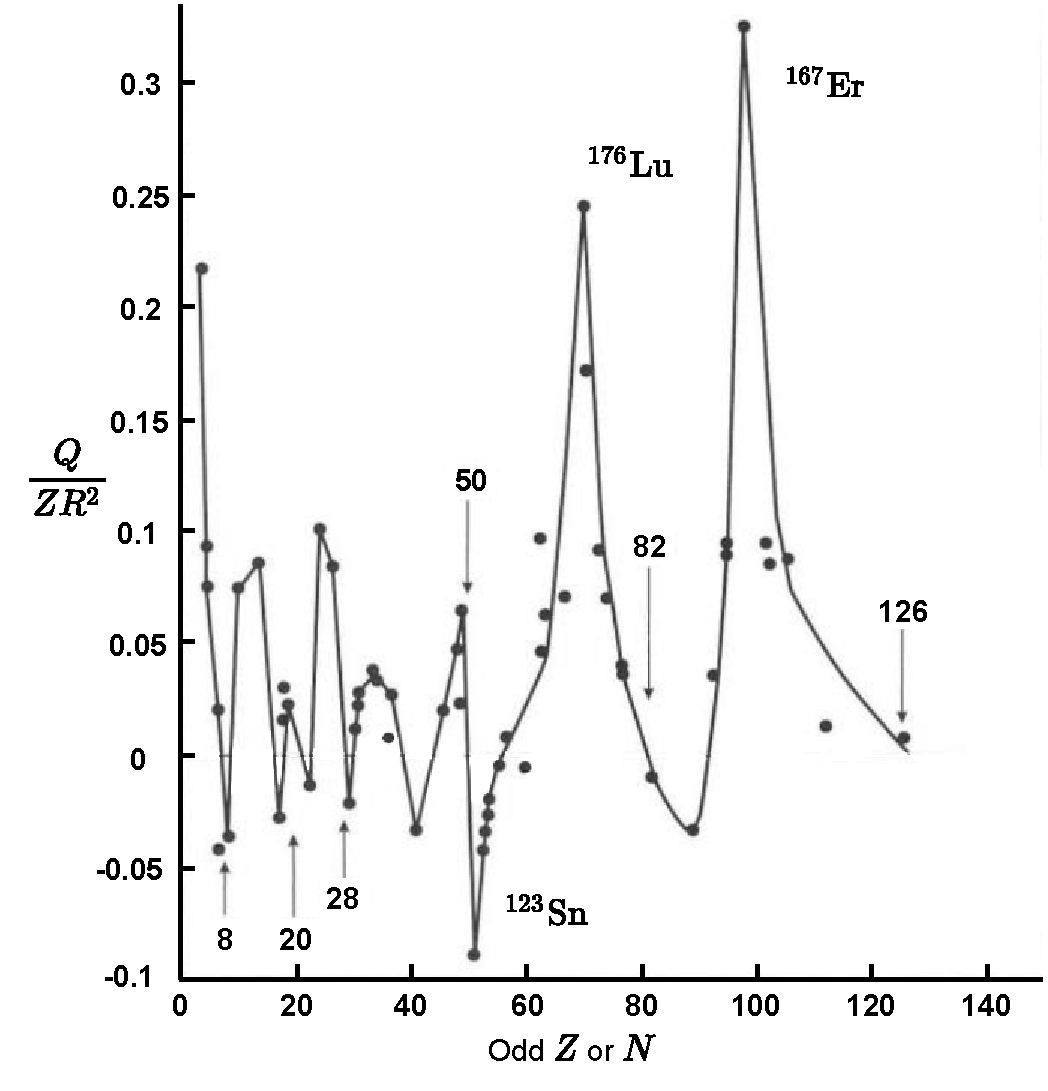
\includegraphics[scale=0.55]{Chapters/Figures/Exp_quadrupoleMoments.pdf}
    \caption{The measured quadrupole moments $Q$ as per Eq. \ref{single-particle-quadrupole-moment}, given in units of $ZR^2$, as function of the odd proton ($Z$) and neutron ($N$) numbers, respectively (arrows signify the magic numbers). Experimental data are taken from Ref. \cite{bertulani2007nuclear}.}
    \label{experimental-Q-odd-nuclei}
\end{figure}

The experimental data for $Q$ (the spectroscopic quadrupole moment in units of \emph{barn} or $\text{b}$) for the lowest $2^+$ states of even-$Z$ and even-$N$ nuclei are graphically represented in Fig. \ref{experimental-quadrupole-2Plus-states}, where both positive and negative values are observed. As already explained, a negative $Q$ value ($Q=-2\ \text{b}$ for nuclei with permanent deformation belonging to the mass range $150\leq A \leq 190$) will correspond to an intrinsic quadrupole moment $Q_0=7\ \text{b}$, which results in deformation parameter $\beta\approx 0.29$. Such values indicate substantial eccentricities of the nuclear matter.
\begin{figure}
    \centering
    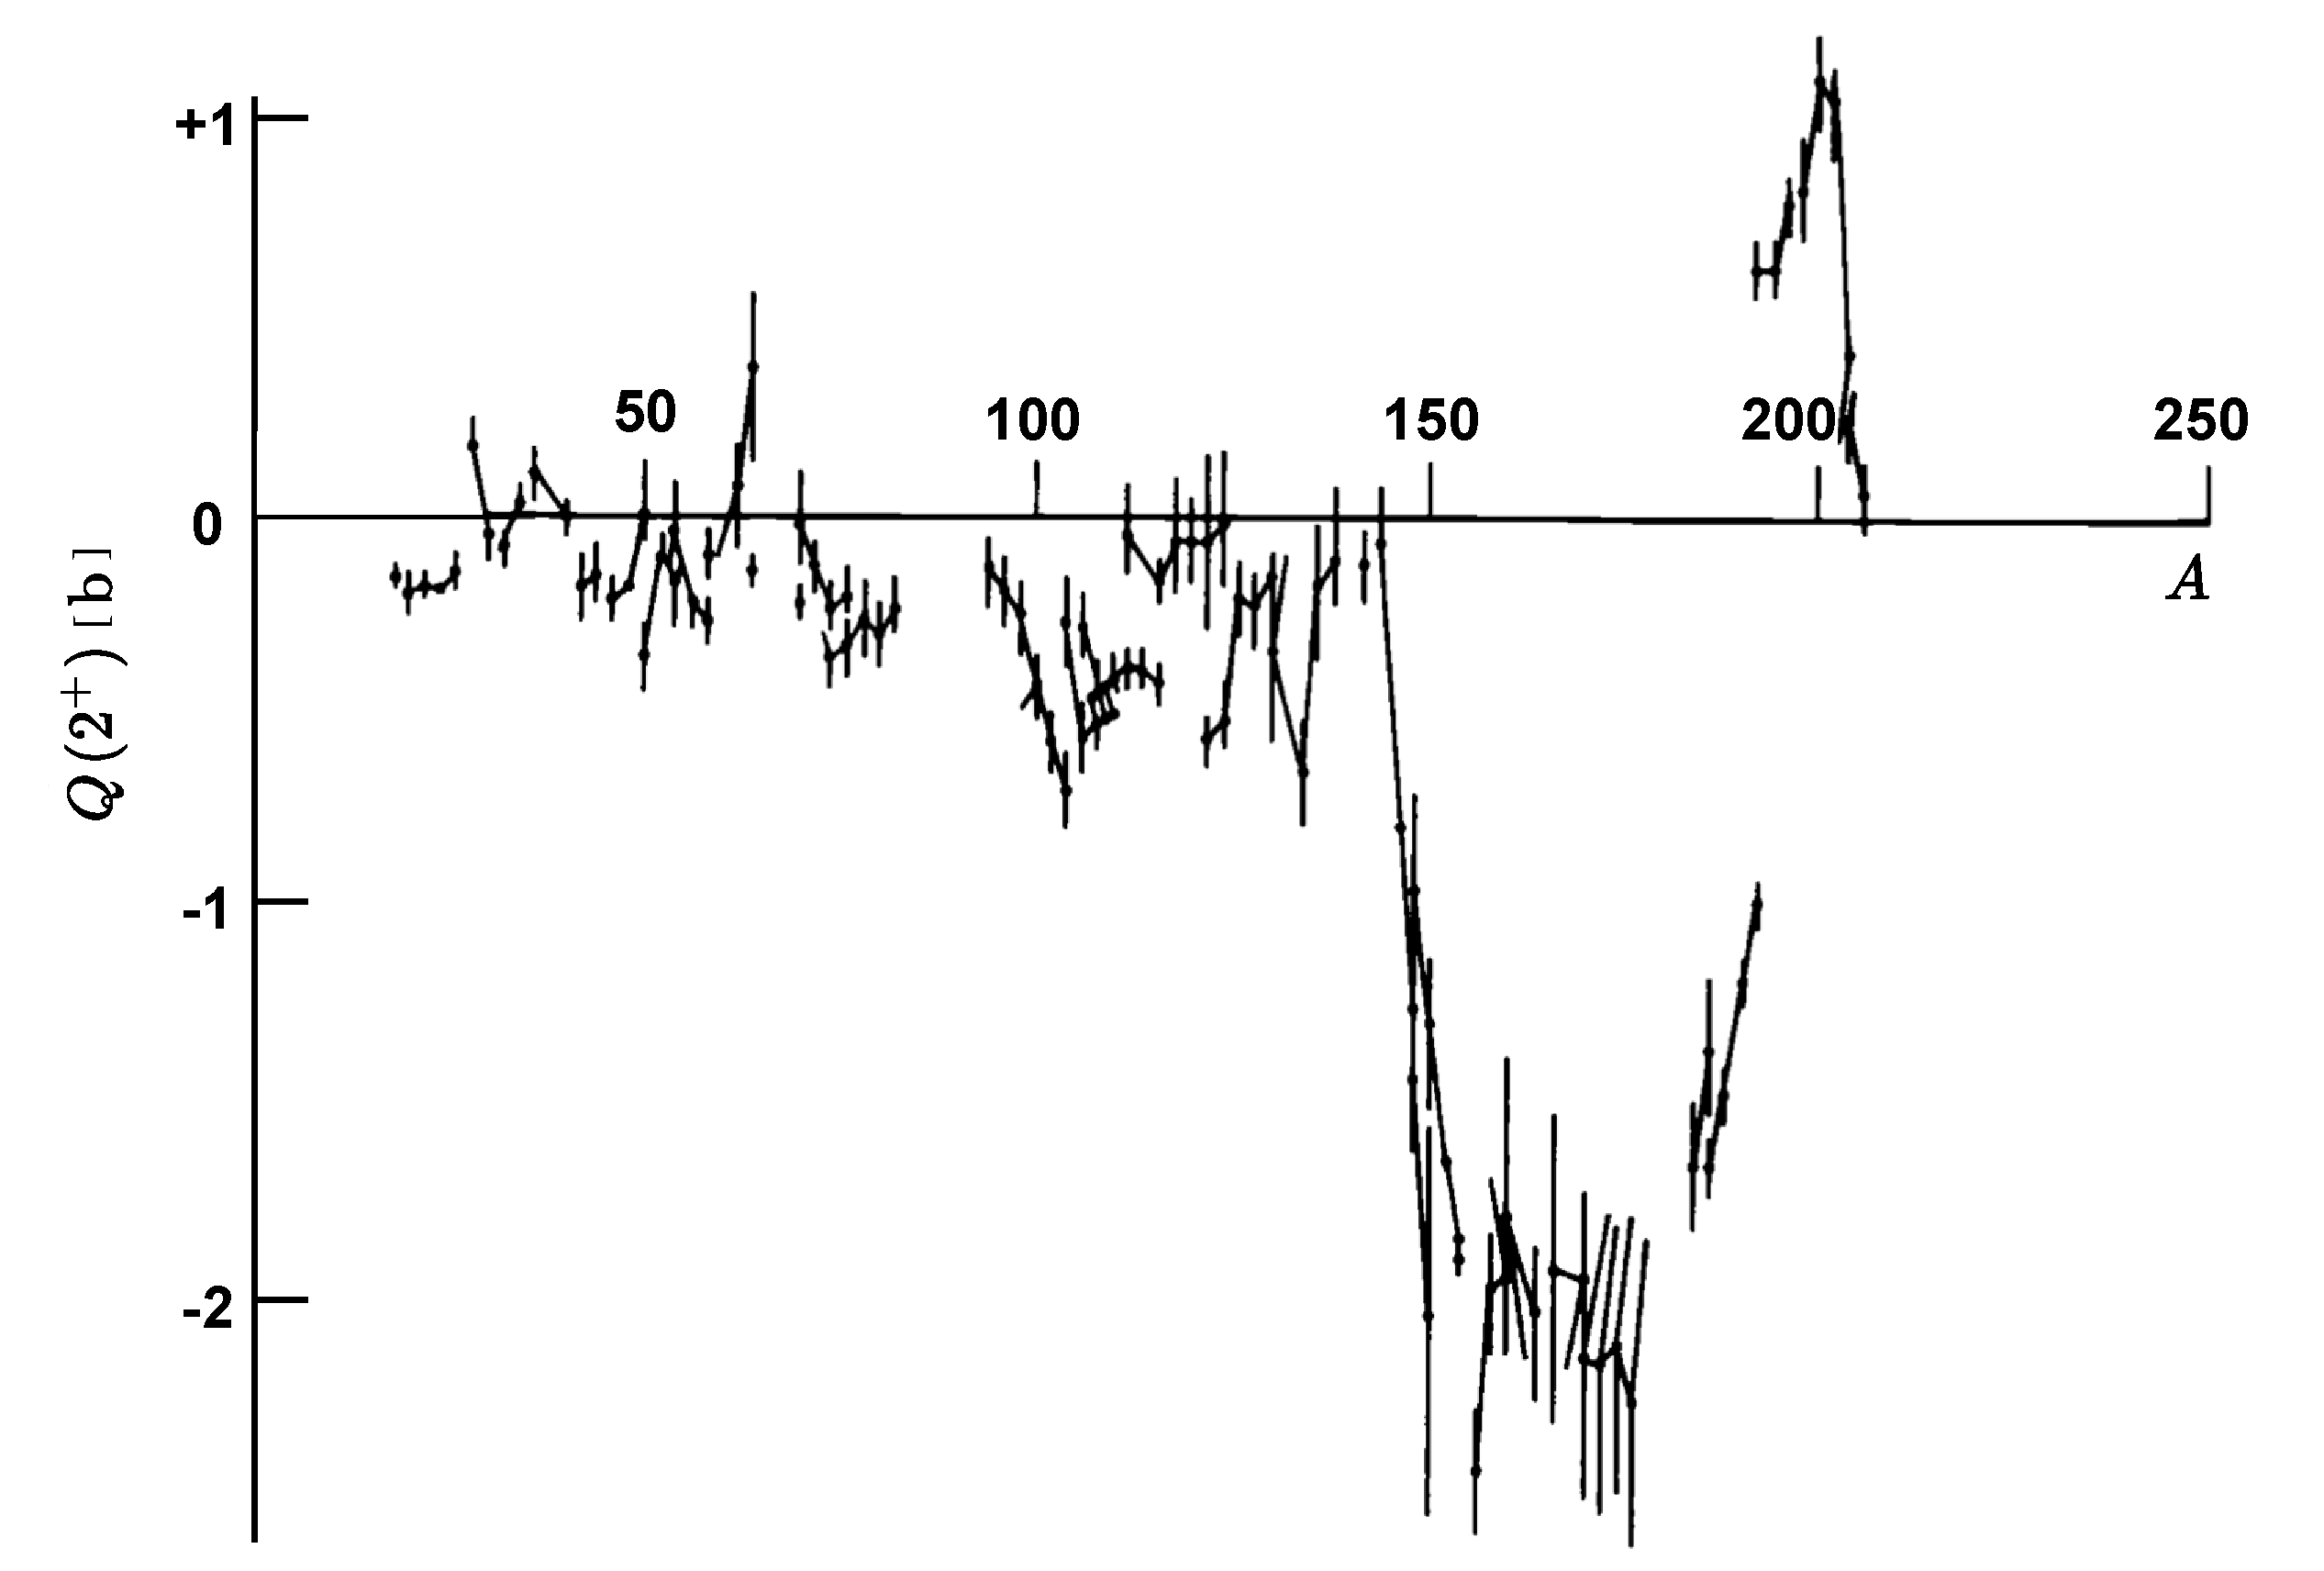
\includegraphics[scale=0.25]{Chapters/Figures/2Plus_spectroscopicQ.pdf}
    \caption{The measured quadrupole moment for the first excited $2^+$ states in even-even nuclei. The expression of $Q$ was defined in Eq. \ref{quadrupole-moment-spectro}. The lines between data-points connect the isotope sequences. The figure was reproduced with the experimental data taken from \cite{krane1991introductory}.}
    \label{experimental-quadrupole-2Plus-states}
\end{figure}

Concluding this chapter, all the relevant models required for understanding the collective phenomena in nuclei were systematically described, starting with the shell model characteristics, then going further with the representation of the single-particle states in deformed nuclei, and finally reaching the collective model. A consistent portrayal for the nuclear rotations and vibrations was given, with the emergence of a general Hamiltonian that describes the nucleus in terms of the $\beta$ and $\gamma$ degrees of freedom. Importance of these two deformation parameters was also emphasized throughout the sections. Lastly, the important quantities indicating collectiveness or deformations were introduced, as they will play a crucial role for testing any newly developed theory.